\chapter{Reproduction in Animals and
Gametogenesis}\label{reproduction-in-animals-and-gametogenesis}

Nearly all animals undergo some form of sexual reproduction. They
produce haploid gametes by meiosis. The smaller, motile gametes are
spermatozoa and the larger, non-motile gametes are ova. The gametes fuse
to form zygotes, which develop via multiple successive mitoses and
differentiation into new individuals.

Some animals are also capable of asexual reproduction. This may take
place through parthenogenesis (from the Greek parthenos, ``virgin'', +
genesis, ``creation''), the development of an embryo from an
unfertilized egg cell. During sexual reproduction, mating with a close
relative (inbreeding) generally leads to reduced biological fitness,
i.e.~the organism's reduced ability to survive and perpetuate its
genetic material. Inbreeding results in more recessive traits
manifesting themselves, as the genomes of pair-mates are more similar.
Animals have evolved numerous diverse mechanisms for avoiding close
inbreeding and promoting out-crossing.

\section{Gametogenesis}\label{gametogenesis}

\href{https://en.wikipedia.org/wiki/Gametogenesis}{Gametogenesis} is a
biological process by which diploid or haploid precursor cells undergo
cell division and differentiation to form mature haploid gametes.
Depending on the biological life cycle of the organism, gametogenesis
occurs by meiotic division of diploid gametocytes into various gametes,
or by mitosis, as we have seen in plants, for example.

Animals produce gametes directly through meiosis in organs called gonads
(testis in males and ovaries in females). Males and females of a species
that reproduces sexually have different forms of gametogenesis

\begin{itemize}
  \tightlist
  \item
  spermatogenesis (male)
  \item
  oogenesis (female)
\end{itemize}

\href{https://en.wikipedia.org/wiki/Spermatogenesis}{Spermatogenesis} is
the process in which an animal produces spermatozoa from spermatogonial
stem cells by way of mitosis and meiosis. The initial cells in this
pathway are called spermatogonia, which yield primary spermatocytes by
mitosis. The primary spermatocyte divides meiotically (Meiosis I) into
two secondary spermatocytes; each secondary spermatocyte divides into
two spermatids by Meiosis II. These develop into mature spermatozoa,
also known as sperm cells. Thus, the primary spermatocyte gives rise to
two cells, the secondary spermatocytes, and the two secondary
spermatocytes by their subdivision produce four spermatozoa.

Spermatozoa are the mature male gametes in many sexually reproducing
organisms. Thus, spermatogenesis is the male version of gametogenesis,
of which the female equivalent is oogenesis. In mammals, it occurs in
the seminiferous tubules of the male testes in a stepwise fashion.
Spermatogenesis is highly dependent upon optimal conditions for the
process to occur correctly, and is essential for sexual reproduction. It
starts at puberty and usually continues uninterrupted until death,
although a slight decrease can be discerned in the quantity of produced
sperm with increase in age

Spermatogenesis takes place within several structures of the male
reproductive system. The initial stages occur within the testes and
progress to the epididymis where the developing gametes mature and are
stored until ejaculation. The seminiferous tubules of the testes are the
starting point for the process, where spermatogonial stem cells adjacent
to the inner tubule wall divide in a centripetal direction---beginning
at the walls and proceeding into the innermost part, or lumen---to
produce immature sperm. Maturation occurs in the epididymis. The
location {[}Testes/Scrotum{]} is specifically important as the process
of spermatogenesis requires a lower temperature to produce viable sperm,
specifically 1-8 °C lower than normal body temperature of 37 °C. For
humans, the entire process of spermatogenesis is variously estimated as
taking between 74 days and approximately 120 days. Including the
transport on ductal system, it takes 3 months. Testes produce 200 to 300
million spermatozoa daily. However, only about half or 100 million of
these become viable sperm.

\href{https://en.wikipedia.org/wiki/Oogenesis}{Oogenesis} is the
differentiation of the ovum (egg cell) into a cell competent to further
development when fertilized. It is developed from the primary oocyte by
maturation. Oogenesis starts with the process of developing oogonia,
which occurs via the transformation of primordial follicles into primary
oocytes, a process called oocytogenesis. Oocytogenesis is complete
either before or shortly after birth. It is commonly believed that, when
oocytogenesis is complete, no additional primary oocytes are created, in
contrast to the male process of spermatogenesis, where gametocytes are
continuously created. In other words, primary oocytes reach their
maximum development at \textasciitilde{}20 weeks of gestational age,
when approximately seven million primary oocytes have been created;
however, at birth, this number has already been reduced to approximately
1-2 million. The succeeding phase of ootidogenesis occurs when the
primary oocyte develops into an ootid. This is achieved by the process
of meiosis. In fact, a primary oocyte is, by its biological definition,
a cell whose primary function is to divide by the process of meiosis.
However, although this process begins at prenatal age, it stops at
prophase I. In late fetal life, all oocytes, still primary oocytes, have
halted at this stage of development, called the dictyate. After
menarche, these cells then continue to develop, although only a few do
so every menstrual cycle. Meiosis I of ootidogenesis begins during
embryonic development, but halts in the diplotene stage of prophase I
until puberty. For those primary oocytes that continue to develop in
each menstrual cycle, however, synapsis occurs and tetrads form,
enabling chromosomal crossover to occur. As a result of meiosis I, the
primary oocyte has now developed into the secondary oocyte and the first
polar body. Immediately after meiosis I, the haploid secondary oocyte
initiates meiosis II. However, this process is also halted at the
metaphase II stage until fertilization, if such should ever occur. When
meiosis II has completed, an ootid and another polar body have now been
created. Synchronously with ootidogenesis, the ovarian follicle
surrounding the ootid has developed from a primordial follicle to a
preovulatory one. Both polar bodies disintegrate at the end of Meiosis
II, leaving only the ootid, which then eventually undergoes maturation
into a mature ovum. The function of forming polar bodies is to discard
the extra haploid sets of chromosomes that have resulted as a
consequence of meiosis.

\section{Embryogenesis and Embryonic
development}\label{embryogenesis-and-embryonic-development}

\href{https://en.wikipedia.org/wiki/Embryogenesis}{Embryogenesis} is the
process by which the embryo forms and develops. In mammals, the term
refers chiefly to early stages of prenatal development, whereas the
terms fetus and fetal development describe later stages. Embryogenesis
starts with the fertilization of the egg cell (ovum) by a sperm cell,
(spermatozoon). Once fertilized, the ovum is referred to as a zygote, a
single diploid cell. The zygote undergoes mitotic divisions with no
significant growth (a process known as cleavage) and cellular
differentiation, leading to development of a multicellular embryo. At
least four initial cell divisions occur, resulting in a dense ball of at
least sixteen cells called the morula. The different cells derived from
cleavage, up to the blastula stage, are called blastomeres. After the
7th cleavage has produced 128 cells, the embryo is called a blastula.
The blastula is usually a spherical layer of cells (the blastoderm)
surrounding a fluid-filled or yolk-filled cavity (the blastocoel).
During gastrulation cells migrate to the interior of the blastula,
subsequently forming two (in diploblastic animals) or three
(triploblastic) germ layers. The embryo during this process is called a
gastrula. The germ layers are referred to as the ectoderm, mesoderm and
endoderm. In diploblastic animals only the ectoderm and the endoderm are
present. In bilateral animals, the blastula develops in one of two ways
that divides the whole animal kingdom into two halves. If in the
blastula the first pore (blastopore) becomes the mouth of the animal, it
is a protostome; if the first pore becomes the anus then it is a
deuterostome. The protostomes include most invertebrate animals, such as
insects, worms and mollusks, while the deuterostomes include the
vertebrates. In due course, the blastula changes into a more
differentiated structure called the gastrula. The gastrula with its
blastopore soon develops three distinct layers of cells (the germ
layers) from which all the bodily organs and tissues then develop:

\begin{itemize}
\tightlist
\item
  The endoderm, the innermost layer, gives a rise to the digestive
  organs, the gills, lungs or swim bladder if present, and kidneys or
  nephrites.
\item
  The mesoderm, the middle layer, gives rise to the muscles, skeleton if
  any, and blood system.
\item
  The ectoderm, the outer layer of cells, gives rise to the nervous
  system, including the brain, and skin or carapace and hair, bristles,
  or scales.
\end{itemize}

\href{https://en.wikipedia.org/wiki/Somitogenesis}{Somitogenesis} is the
process by which somites (primitive segments) are produced. These
segmented tissue blocks differentiate into skeletal muscle, vertebrae,
and dermis of all vertebrates. At some point after the different germ
layers are defined, organogenesis begins. The first stage in vertebrates
is called neurulation, where the neural plate folds forming the neural
tube. Other common organs or structures that arise at this time include
the heart and somites, but from now on embryogenesis follows no common
pattern among the different taxa of the animal kingdom. In most animals,
organogenesis along with morphogenesis will result in a larva. The
hatching of the larva, which must then undergo metamorphosis, marks the
end of embryonic development.

\section{Comparative embryology}\label{comparative-embryology}

\href{https://en.wikipedia.org/wiki/Comparative_embryology}{Comparative
embryology} is the branch of embryology that compares and contrasts
embryos of different species. It is used to show how all animals are
related. Many things are compared (such as whether or not the organism
has a notochord or gill arches). Many components go into comparative
embryology, and much information about the developmental similarities
between species can be taken from its study, from which many conclusions
can be drawn. These similarities among species are called homologous
structures, which are structures that have the same or similar function
and mechanism, having evolved from a common ancestor. The goal of
comparative embryology is to make sense of how an embryo develops, and
of how all animals are related. Comparative embryology also supports
evolutionary theory, in the sense that all vertebrates develop
similarly. The conclusion is that all vertebrates must have a common
ancestor.

\section{View Prepared Slides}\label{view-prepared-slides-2}

\section{Starfish embryology}\label{starfish-embryology}

\begin{enumerate}
\def\labelenumi{\arabic{enumi}.}
\tightlist
\item
  Starfish development slide (Figure \ref{fig:development})

  \begin{itemize}
  \tightlist
  \item
    Locate: unfertilized egg, fertilized egg, 2-cell, 4-cell, 8-cell,
    morula, blastula, early gastrula, late gastrula, bipinnaria larva.
    In a late gastrula, locate the primary germ layers (ectoderm,
    mesoderm, endoderm), archenteron (primitive gut), blastopore and
    blastocoel.
  \end{itemize}
\end{enumerate}

\begin{figure}

{\centering 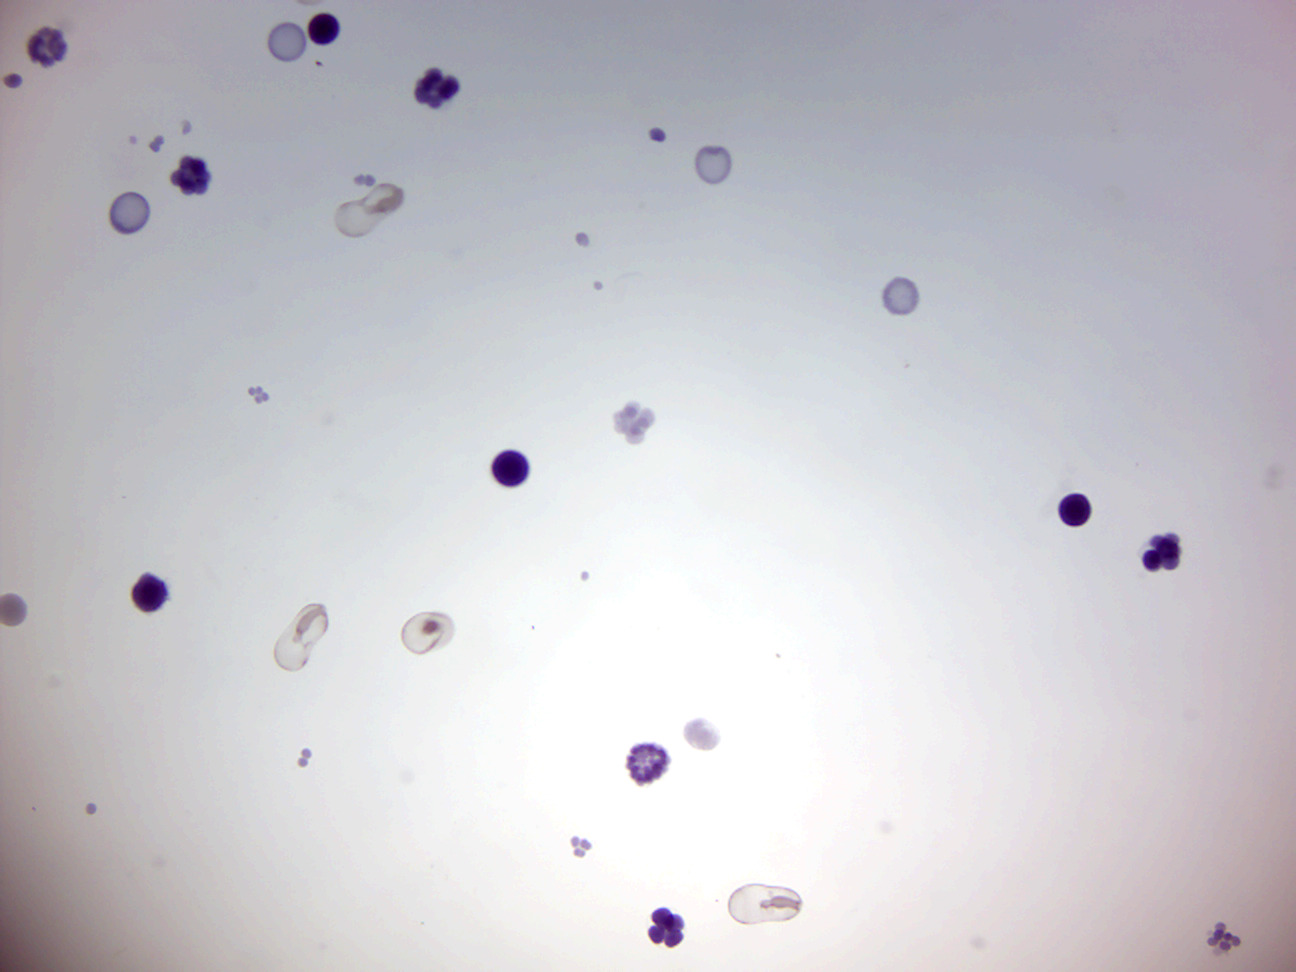
\includegraphics[width=0.7\linewidth]{./figures/development/starfish_development}

}

\caption{Starfish development.}\label{fig:development}
\end{figure}

\section{Frog embryology}\label{frog-embryology}

\begin{enumerate}
\def\labelenumi{\arabic{enumi}.}
\tightlist
\item
  Frog early cleavage (Figure \ref{fig:cleavage})
\begin{itemize}
  \tightlist
  \item
  Count the cells in
  this early from embryo.
  \end{itemize}
\item
  Frog blastula (Figure \ref{fig:blastula})
\item
  Frog gastrulation: yolk plug stage (Figure \ref{fig:plug})
\begin{itemize}
  \tightlist
  \item
  Locate:
  yolk plug, ectoderm, endoderm, archenteron (gastrocoel)
\end{itemize}

\item
  Frog gastrula (Figure \ref{fig:gastrula})
\item
  Frog early neural groove x.s. (Figure \ref{fig:groove})

\begin{itemize}
\tightlist
  \item
  Locate
  neural groove, ectoderm, endoderm, mesoderm, archenteron, location of
  presumptive notochord
\end{itemize}

\item
  Frog late neural tube x.s. (Figure \ref{fig:tube})
\begin{itemize}
    \tightlist
  \item
  Locate: neural
  tube, ectoderm, endoderm, mesoderm, coelom, archenteron, notochord
\end{itemize}
\end{enumerate}

\begin{figure}

{\centering 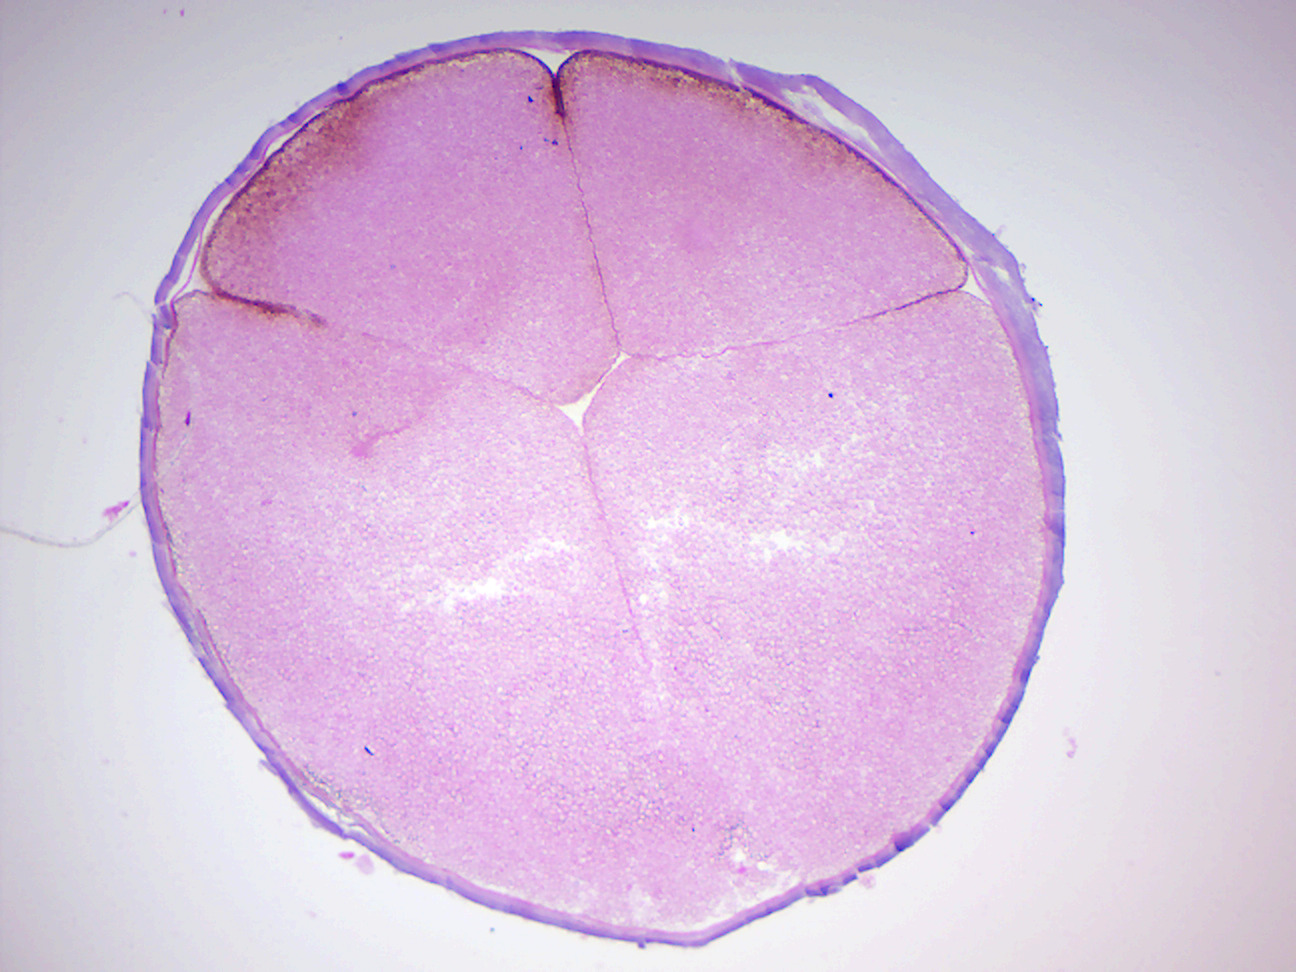
\includegraphics[width=0.7\linewidth]{./figures/development/frog_early_cleavage}

}

\caption{Frog early cleavage.}\label{fig:cleavage}
\end{figure}

\begin{figure}

{\centering 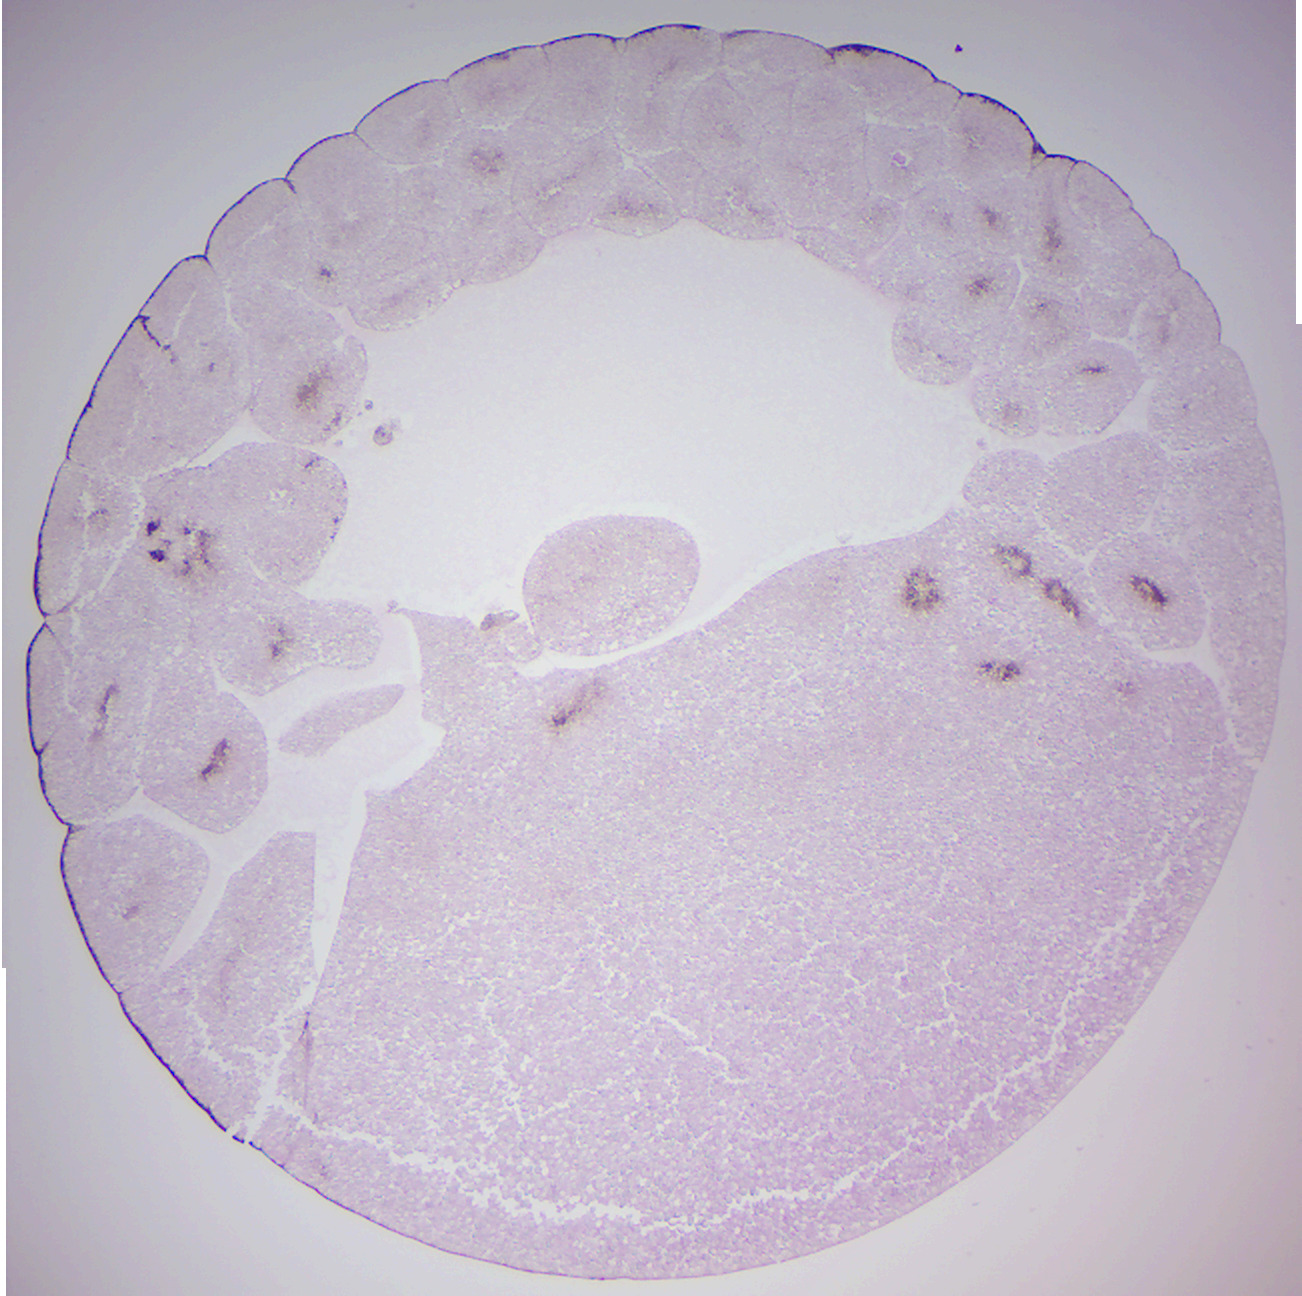
\includegraphics[width=0.7\linewidth]{./figures/development/frog_blastula}

}

\caption{Frog blastula.}\label{fig:blastula}
\end{figure}

\begin{figure}

{\centering 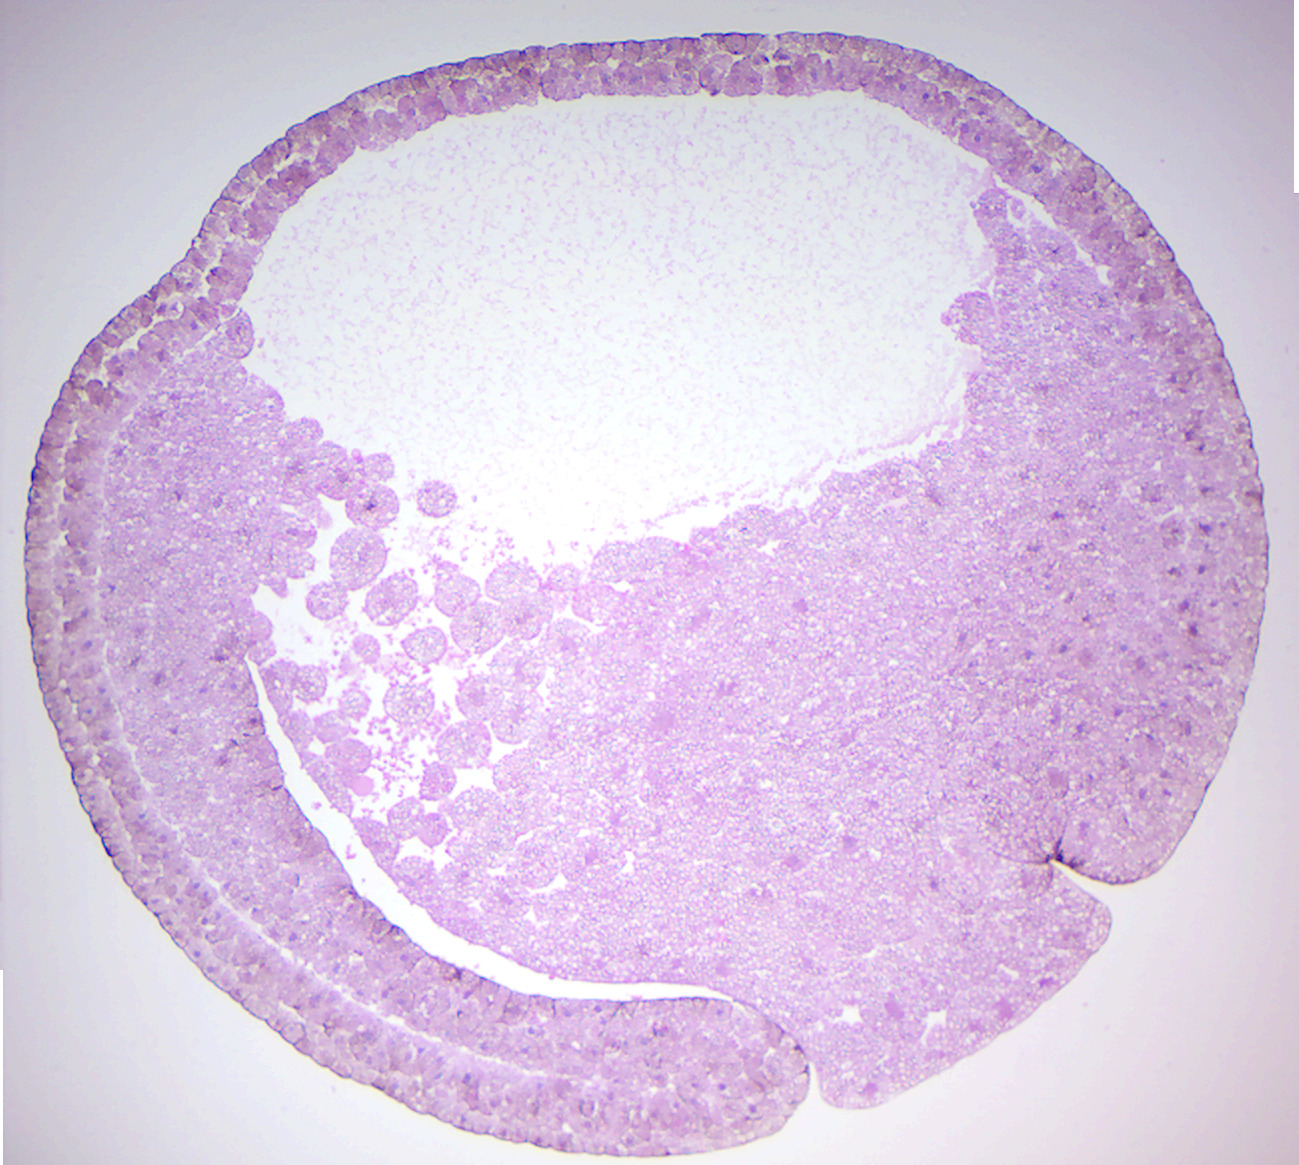
\includegraphics[width=0.7\linewidth]{./figures/development/frog_gastrula_yolk_plug}

}

\caption{Frog gastrulation with yolk plug.}\label{fig:plug}
\end{figure}

\begin{figure}

{\centering 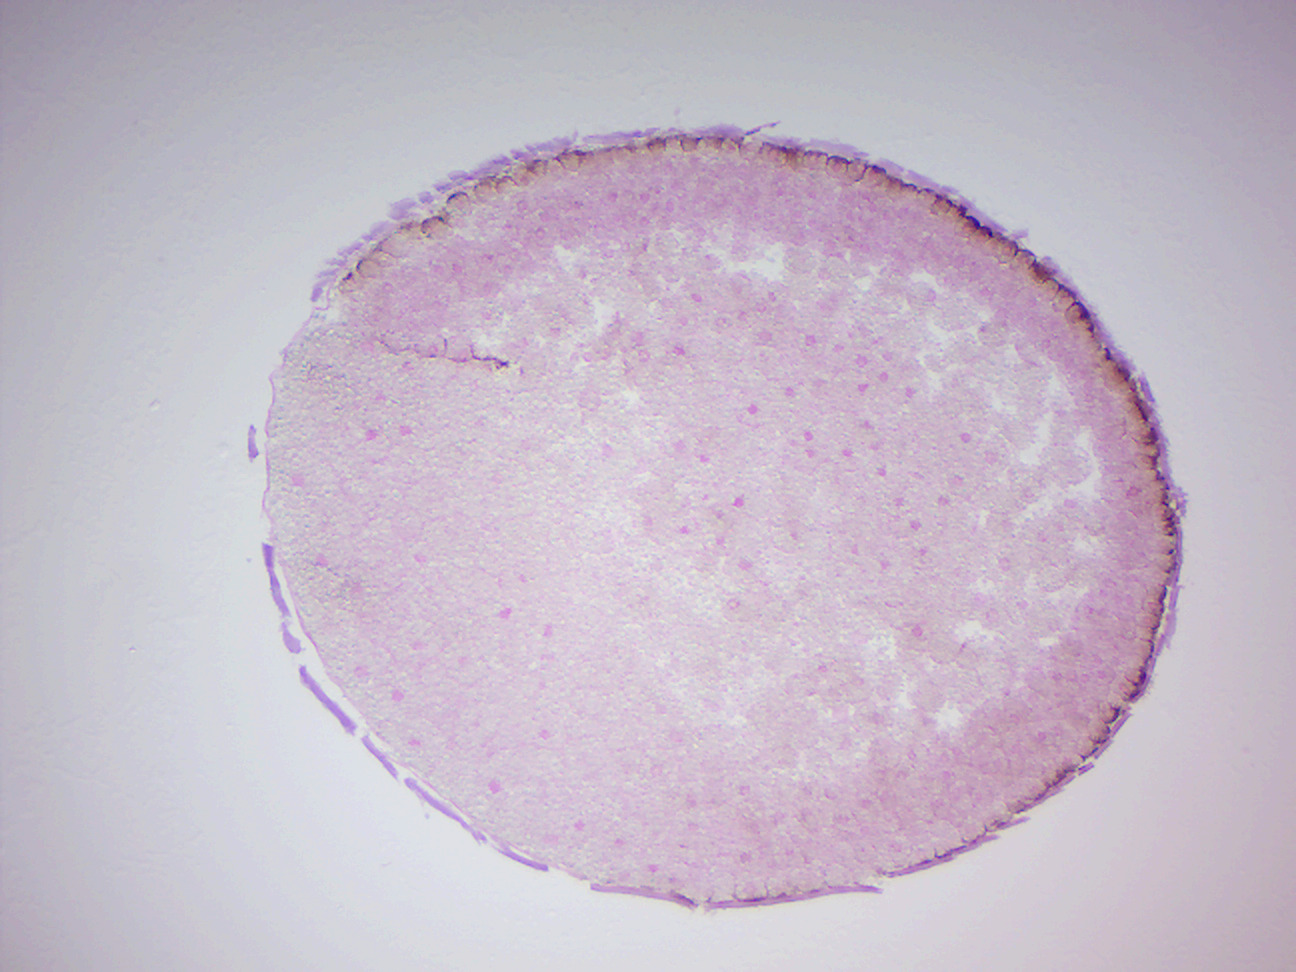
\includegraphics[width=0.7\linewidth]{./figures/development/frog_gastrula}

}

\caption{Frog gastrula.}\label{fig:gastrula}
\end{figure}

\begin{figure}

{\centering 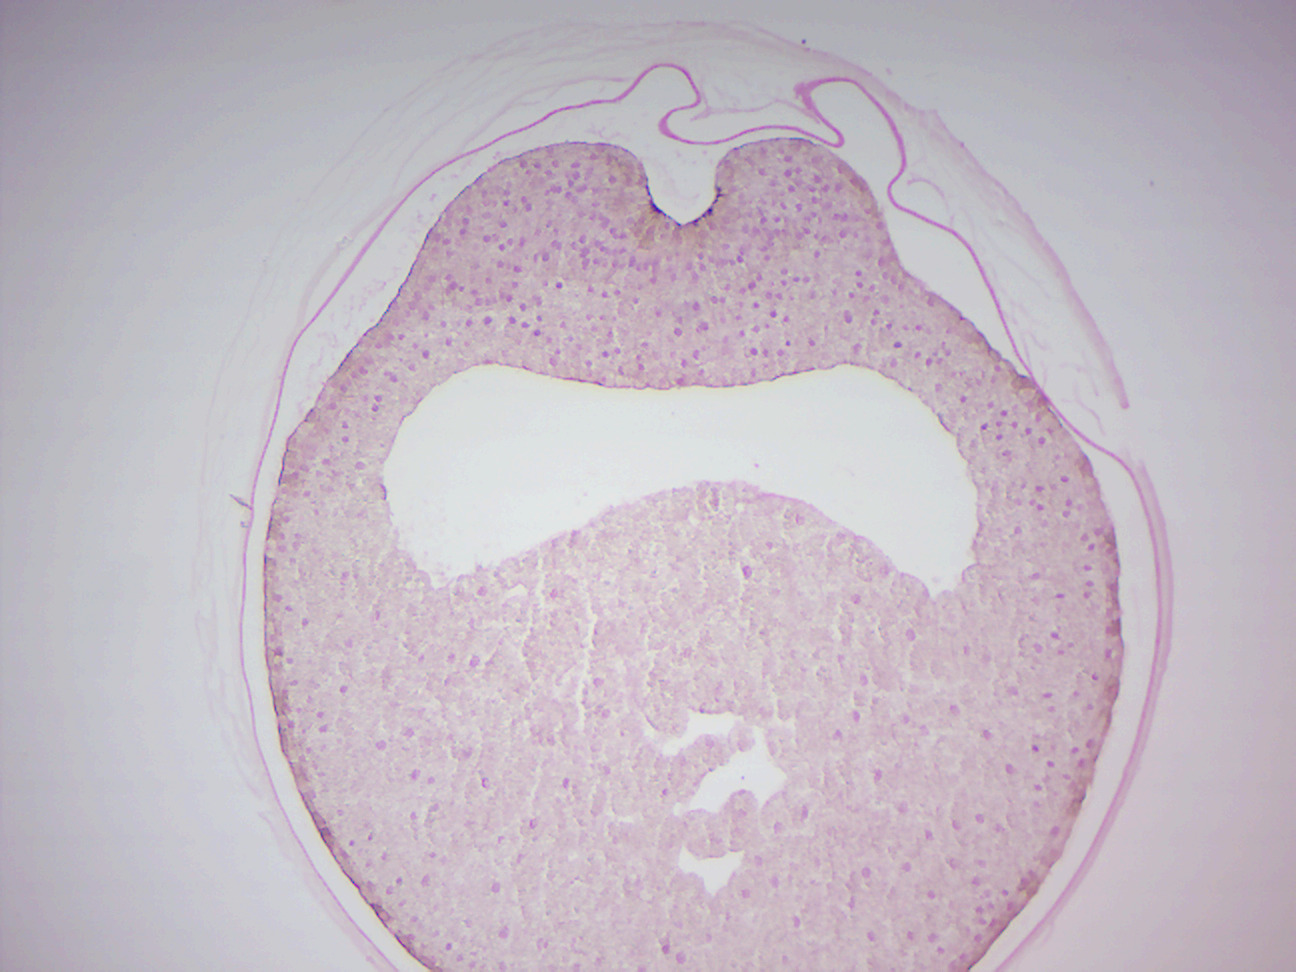
\includegraphics[width=0.7\linewidth]{./figures/development/frog_neural_groove}

}

\caption{Frog neural groove.}\label{fig:groove}
\end{figure}

\begin{figure}

{\centering 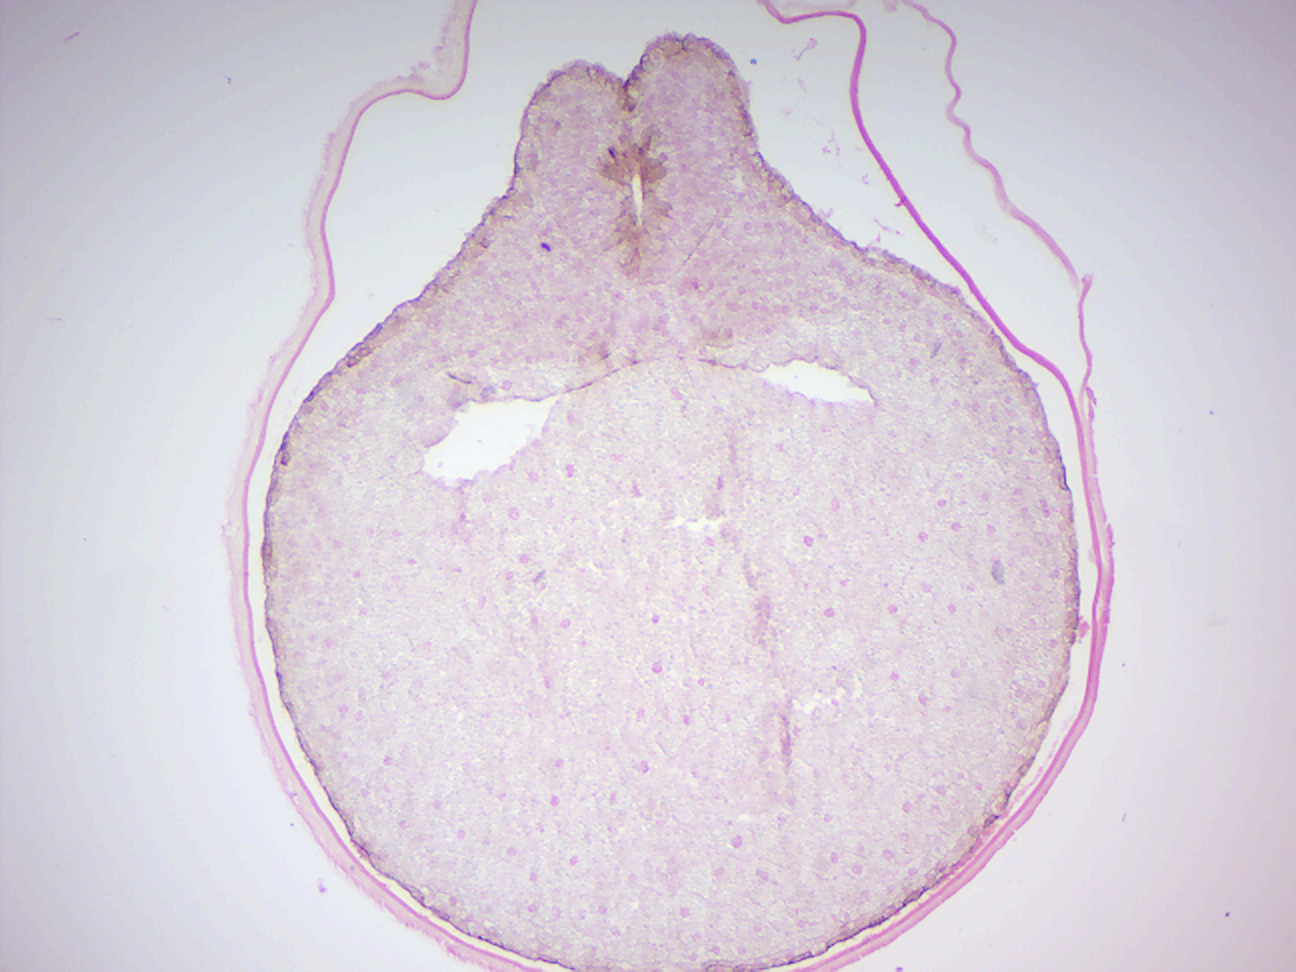
\includegraphics[width=0.7\linewidth]{./figures/development/frog_neural_tube}

}

\caption{Frog neural tube.}\label{fig:tube}
\end{figure}

\section{Chicken embryology}\label{chicken-embryology}

\BeginKnitrBlock{rmdcaution}
\textbf{Notice that these slides are very thick, since they contain
whole mounts (w.m.) of chicken embryos. Use only the 4× (low power)
objective of your microscope to avoid crushing these slides.}
\EndKnitrBlock{rmdcaution}

\begin{enumerate}
\def\labelenumi{\arabic{enumi}.}
\tightlist
\item
  Chick embryo 33 hrs (Figure \ref{fig:chick33h}).

\begin{itemize}
\tightlist
  \item
  Locate: head
  amniotic fold, forebrain, midbrain, hindbrain, heart, somites, neural
  tube. What structures will develop from the somites later?
\end{itemize}
\item
  Chick embryo 48 hrs (Figure \ref{fig:chick48h}).
  \begin{itemize}
  \tightlist
    \item
  Locate: same
  structures as above plus: optic cup with lens, ventricle and atrium of
  the heart, auditory vesicle, tail, and tail amniotic fold, notochord.
\end{itemize}
\item
  Chick embryo 72 hrs (Figure \ref{fig:chick72h}).
  \begin{itemize}
  \tightlist
    \item
  Locate: same
  structures as above plus; allantois, hind limb bud.
  \end{itemize}
\item
  Chick Embryo 96 hrs (Figure \ref{fig:chick96h}).
  \begin{itemize}
  \tightlist
    \item
  Locate: same
  structures as above.
  \end{itemize}
\end{enumerate}

\begin{figure}

{\centering 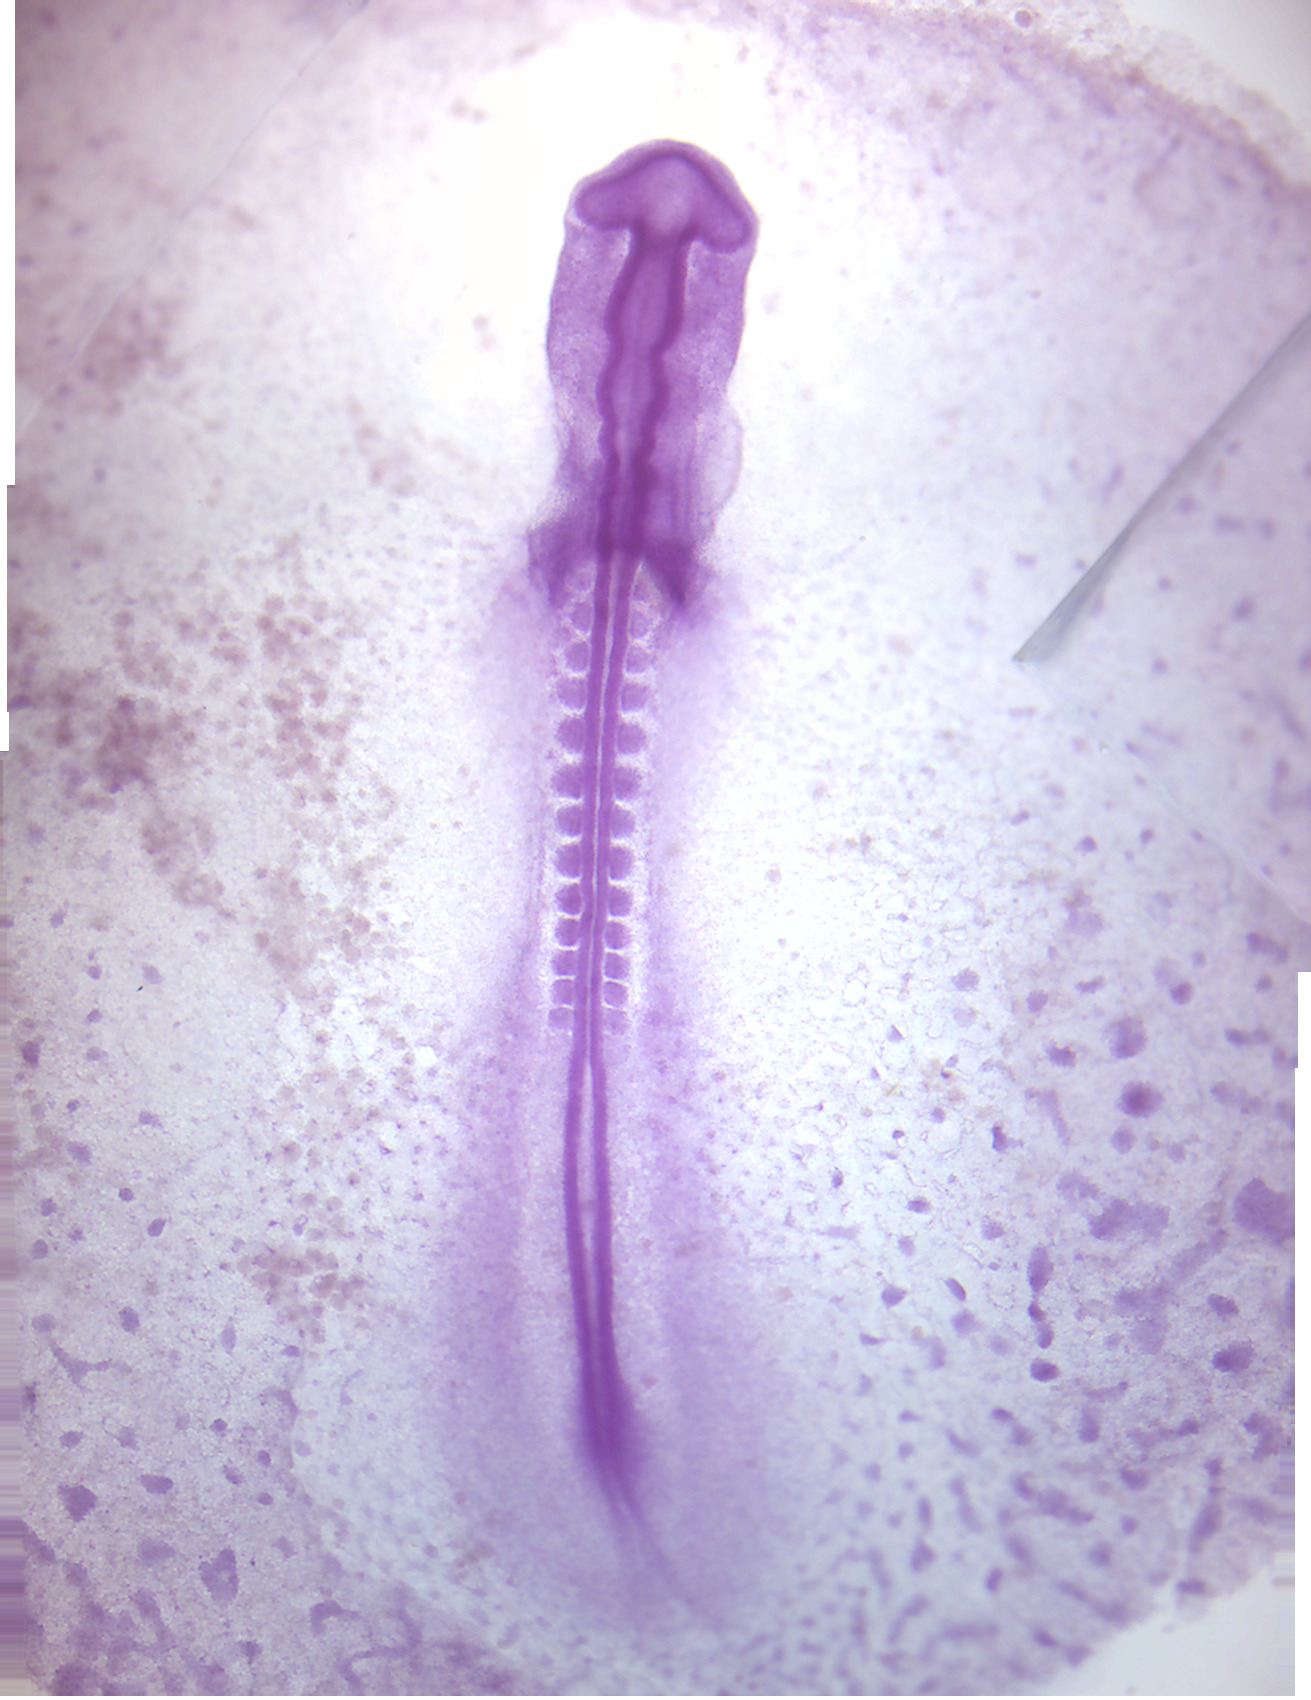
\includegraphics[width=0.7\linewidth]{./figures/development/chick_33h}

}

\caption{Chick embryo at 33 hours.}\label{fig:chick33h}
\end{figure}

\begin{figure}

{\centering 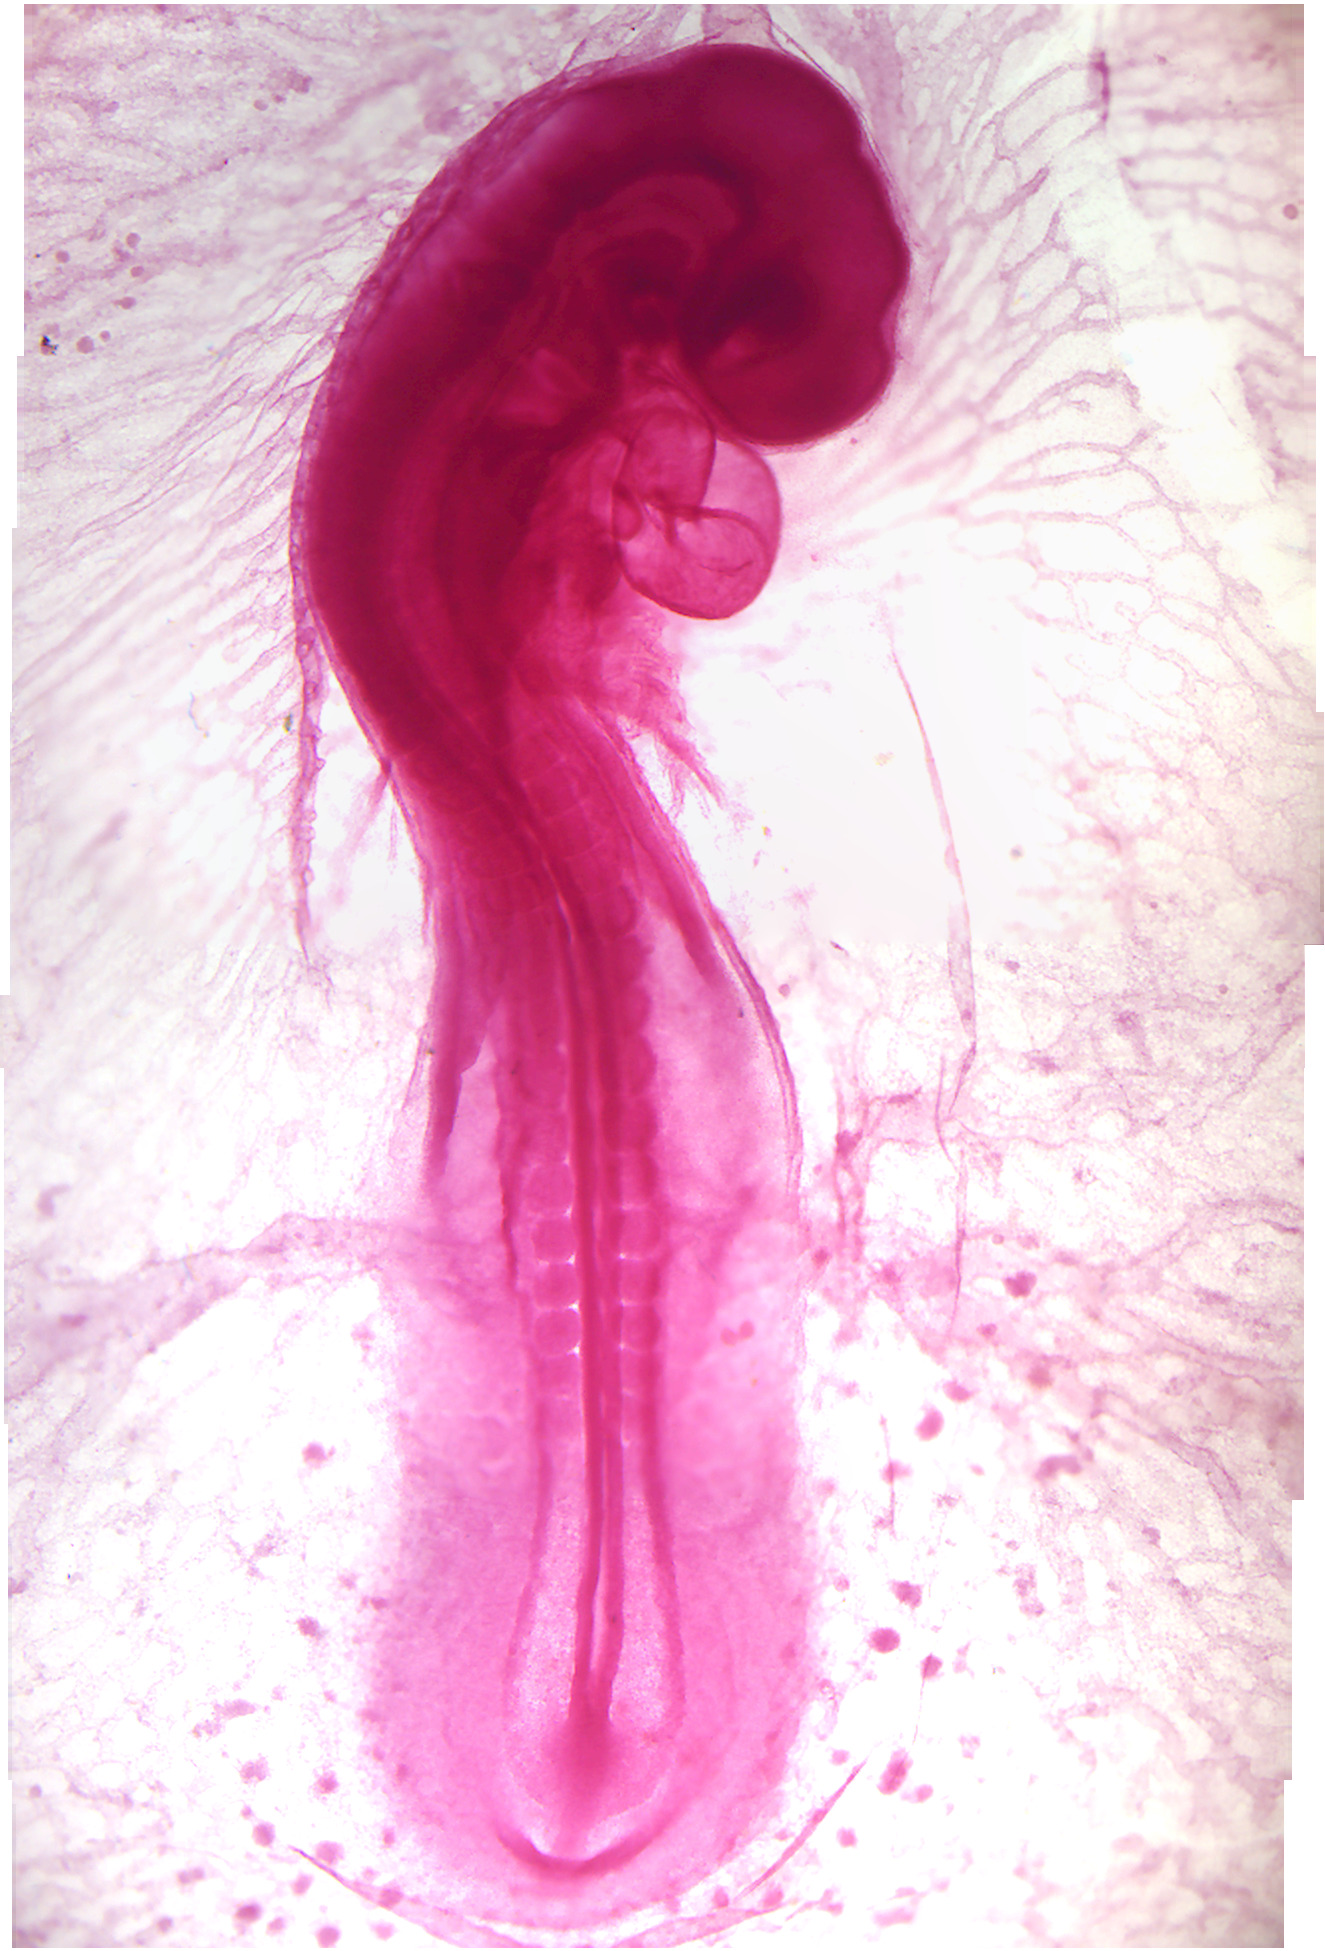
\includegraphics[width=0.7\linewidth]{./figures/development/chick_48h}

}

\caption{Chick embryo at 48 hours.}\label{fig:chick48h}
\end{figure}

\begin{figure}

{\centering 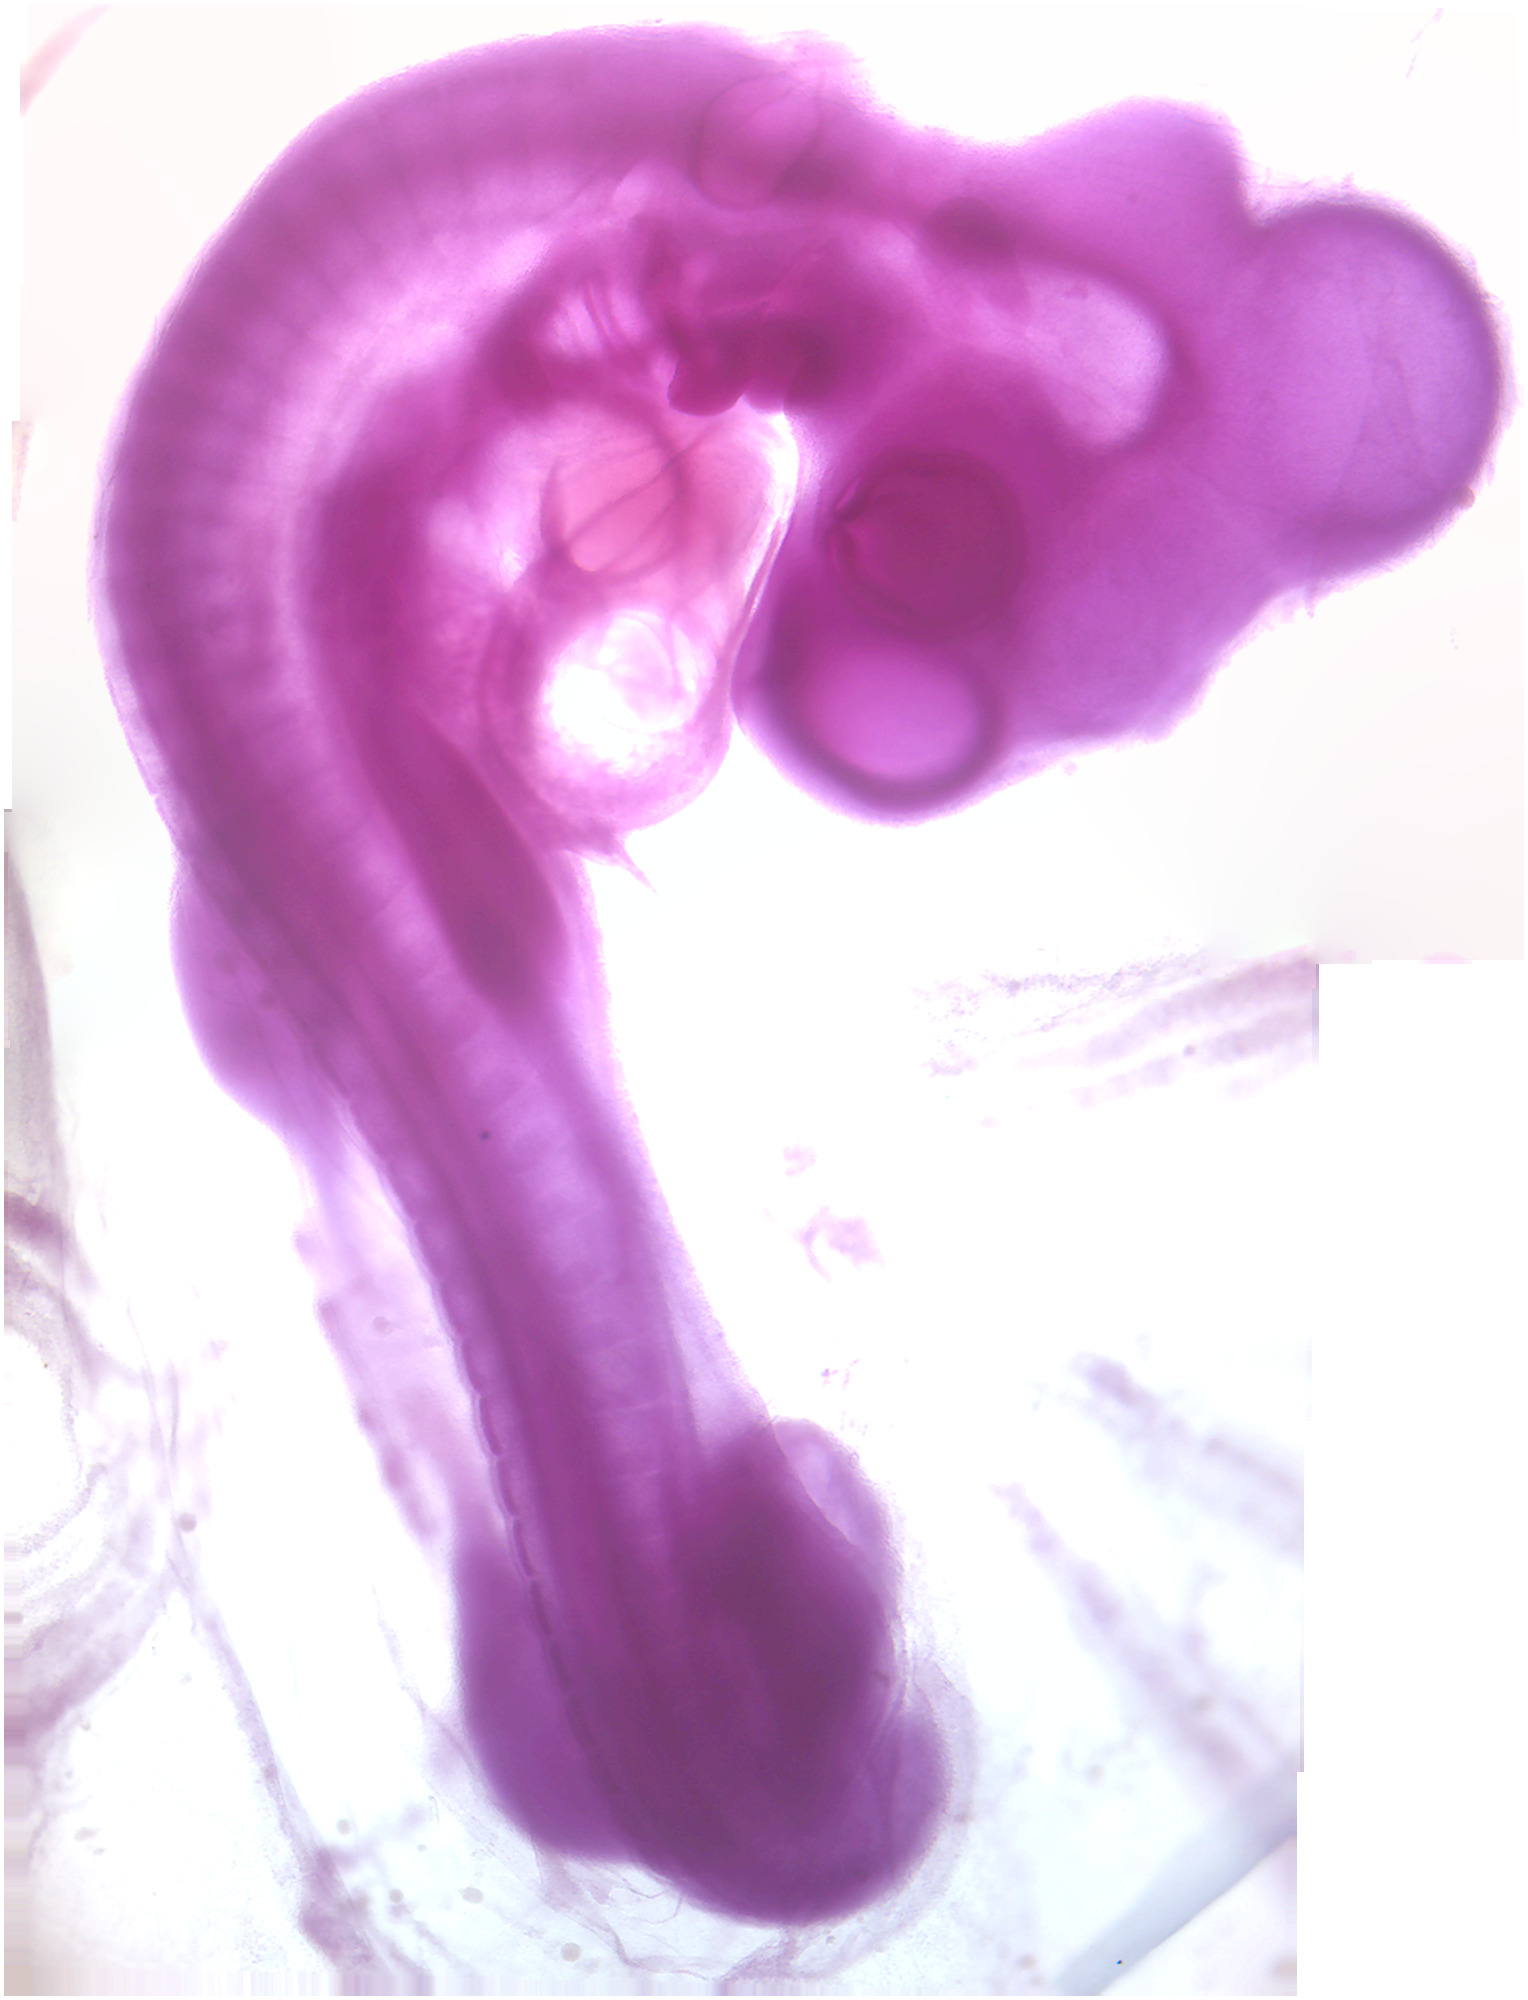
\includegraphics[width=0.7\linewidth]{./figures/development/chick_72h}

}

\caption{Chick embryo at 72 hours.}\label{fig:chick72h}
\end{figure}

\begin{figure}

{\centering 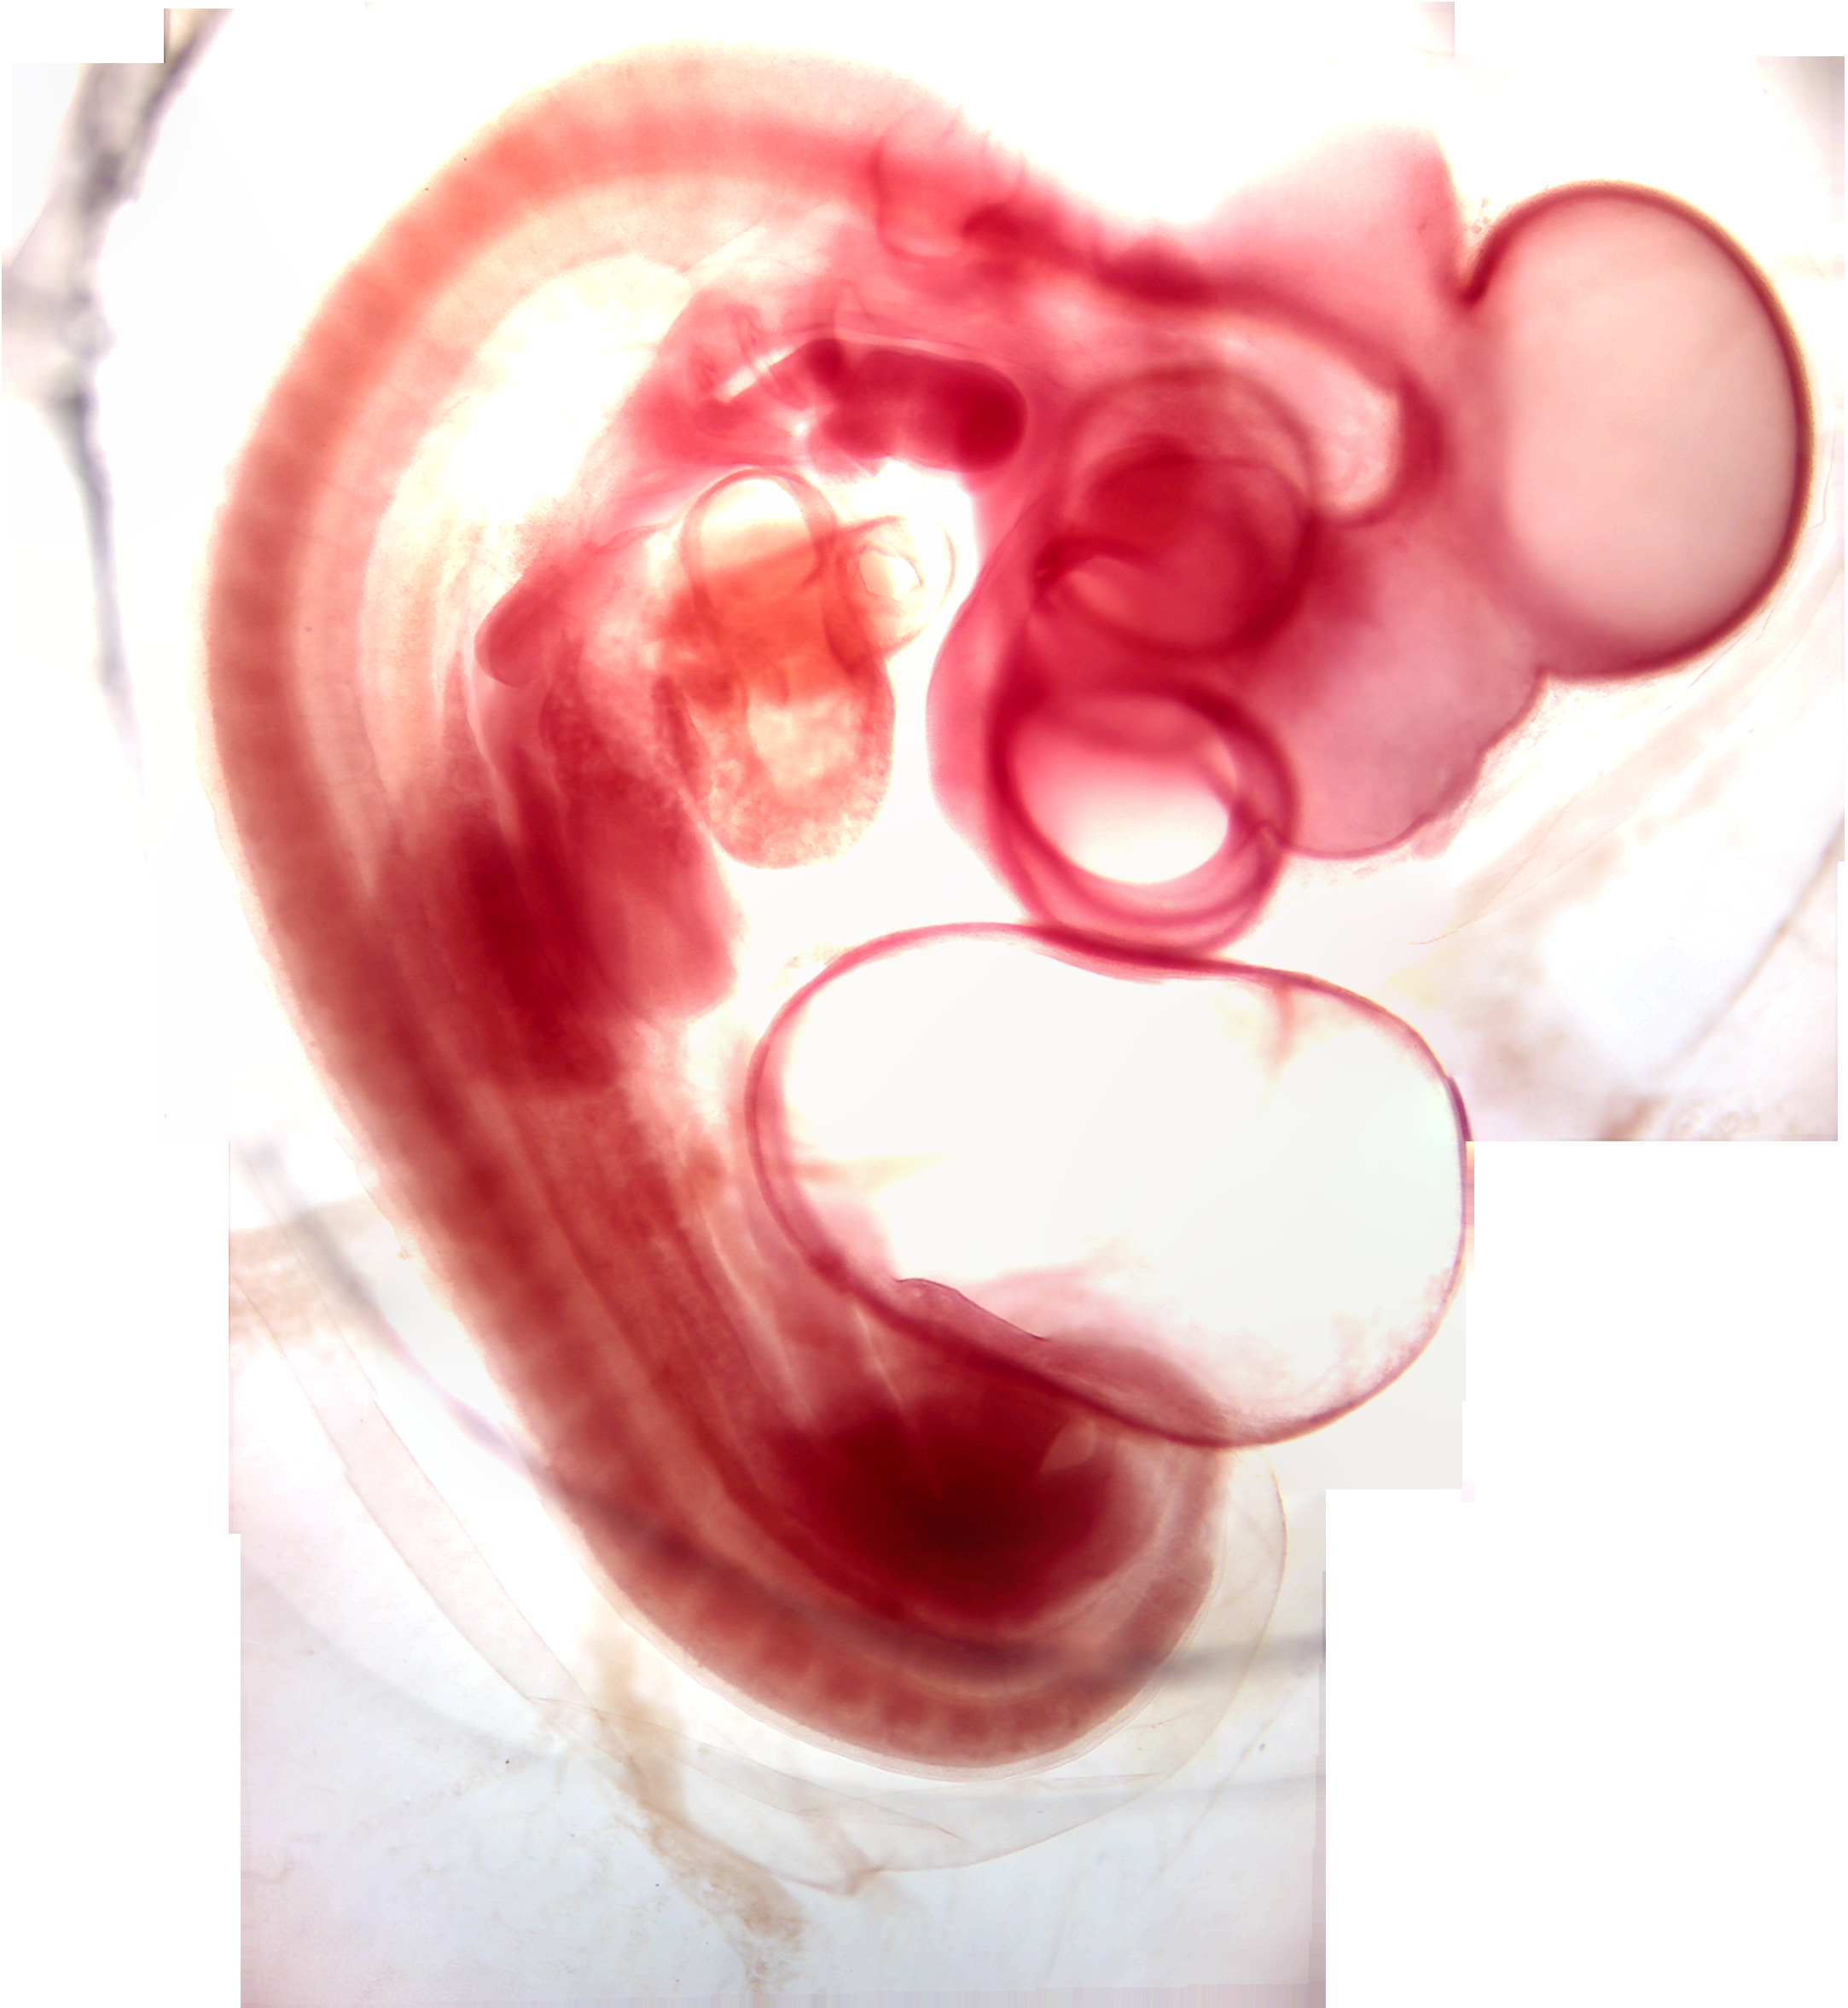
\includegraphics[width=0.7\linewidth]{./figures/development/chick_96h}

}

\caption{Chick embryo at 96 hours.}\label{fig:chick96h}
\end{figure}

\section{Mammalian reproductive organs and
gametes}\label{mammalian-reproductive-organs-and-gametes}

\begin{enumerate}
\def\labelenumi{\arabic{enumi}.}
\tightlist
\item
  Cat ovary (Figure \ref{fig:ovary})
\begin{itemize}
  \item
  Identify primary, secondary and
  Graffian follicles
\end{itemize}
\item
  Graafian follicle (Figure \ref{fig:graafian}).
\item
  Cat ovary Corpus Luteum
  \begin{itemize}
    \item
  Locate corpus luteum
\end{itemize}
\item
  Uterus (Figure \ref{fig:uterus})

\begin{itemize}
  \item
  Identfy: endometrium, myometrium,
  perimetrium
\end{itemize}

\item
  Monkey testis (Figure \ref{fig:monkeytestis})

\begin{itemize}
  \item
  Locate: semimiferous
  tubules, spermatozoa
\end{itemize}

\item
  Human testis (Figure \ref{fig:humantestis})
  \begin{itemize}
    \item
    Locate: semimiferous
    tubules, spermatozoa
  \end{itemize}
\item
  Human sperm smear (Figure \ref{fig:sperm})

\begin{itemize}
  \item
  Identify: sperm, sperm
  head, sperm neck and sperm tail
\end{itemize}


\end{enumerate}

\begin{figure}

{\centering 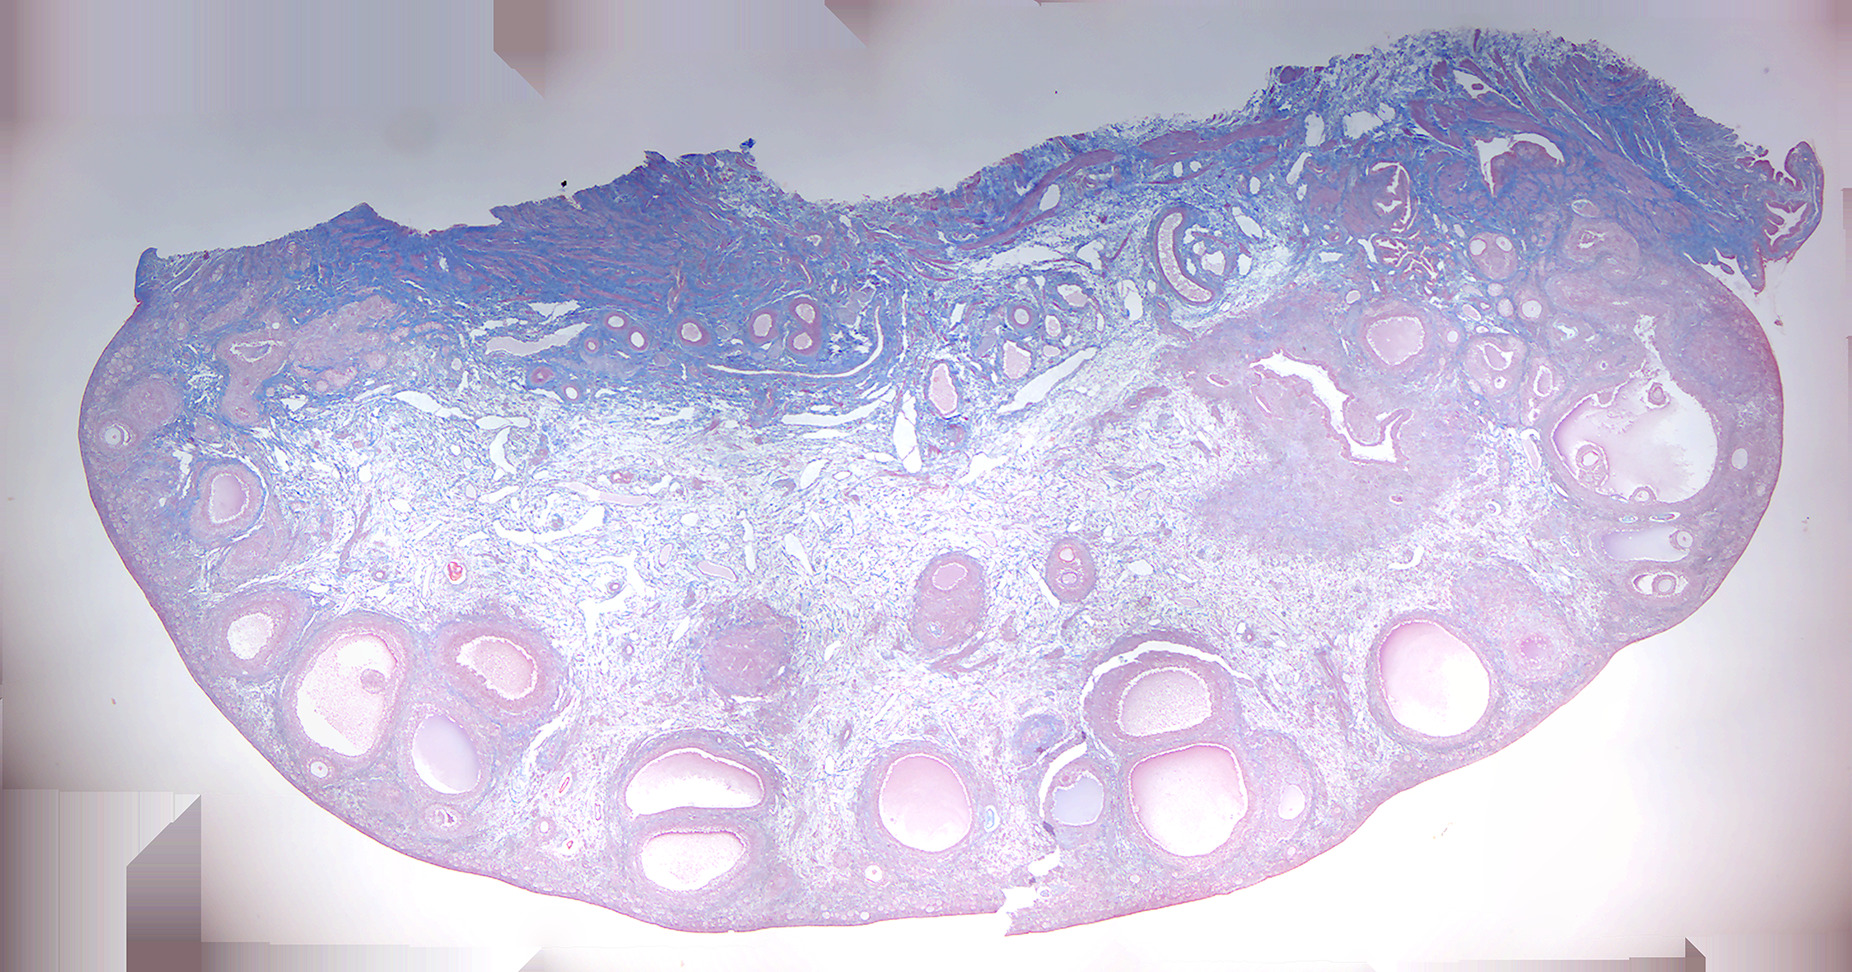
\includegraphics[width=0.7\linewidth]{./figures/development/cat_ovary}

}

\caption{Cat ovary.}\label{fig:ovary}
\end{figure}

\begin{figure}

{\centering 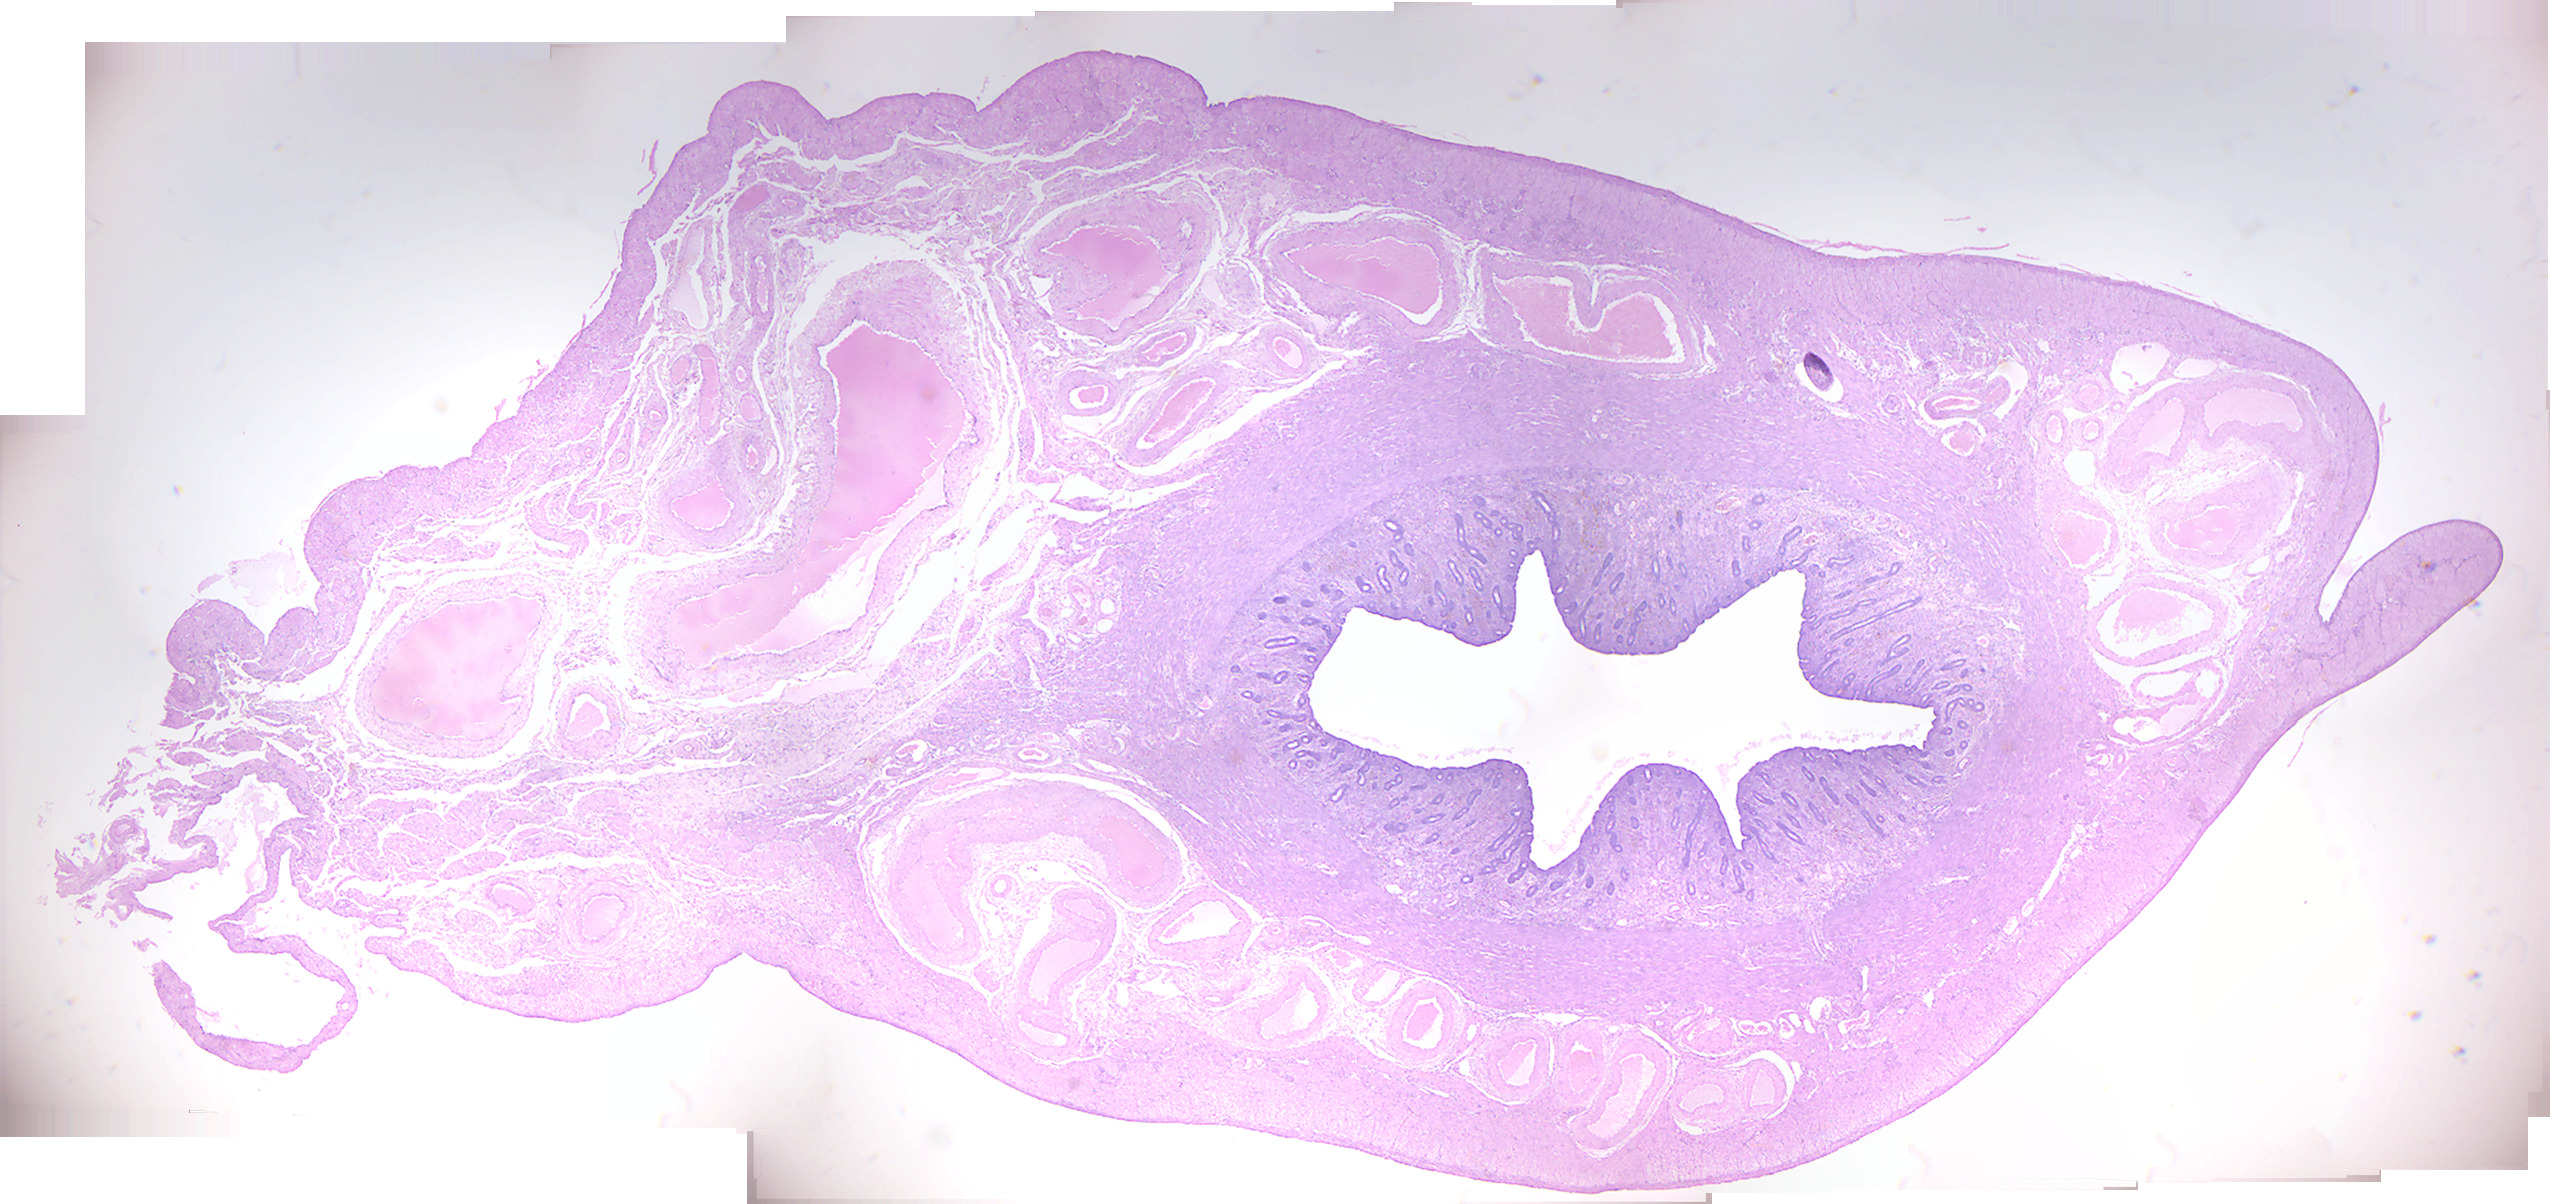
\includegraphics[width=0.7\linewidth]{./figures/development/uterus}

}

\caption{Uterus.}\label{fig:uterus}
\end{figure}

\begin{figure}

{\centering 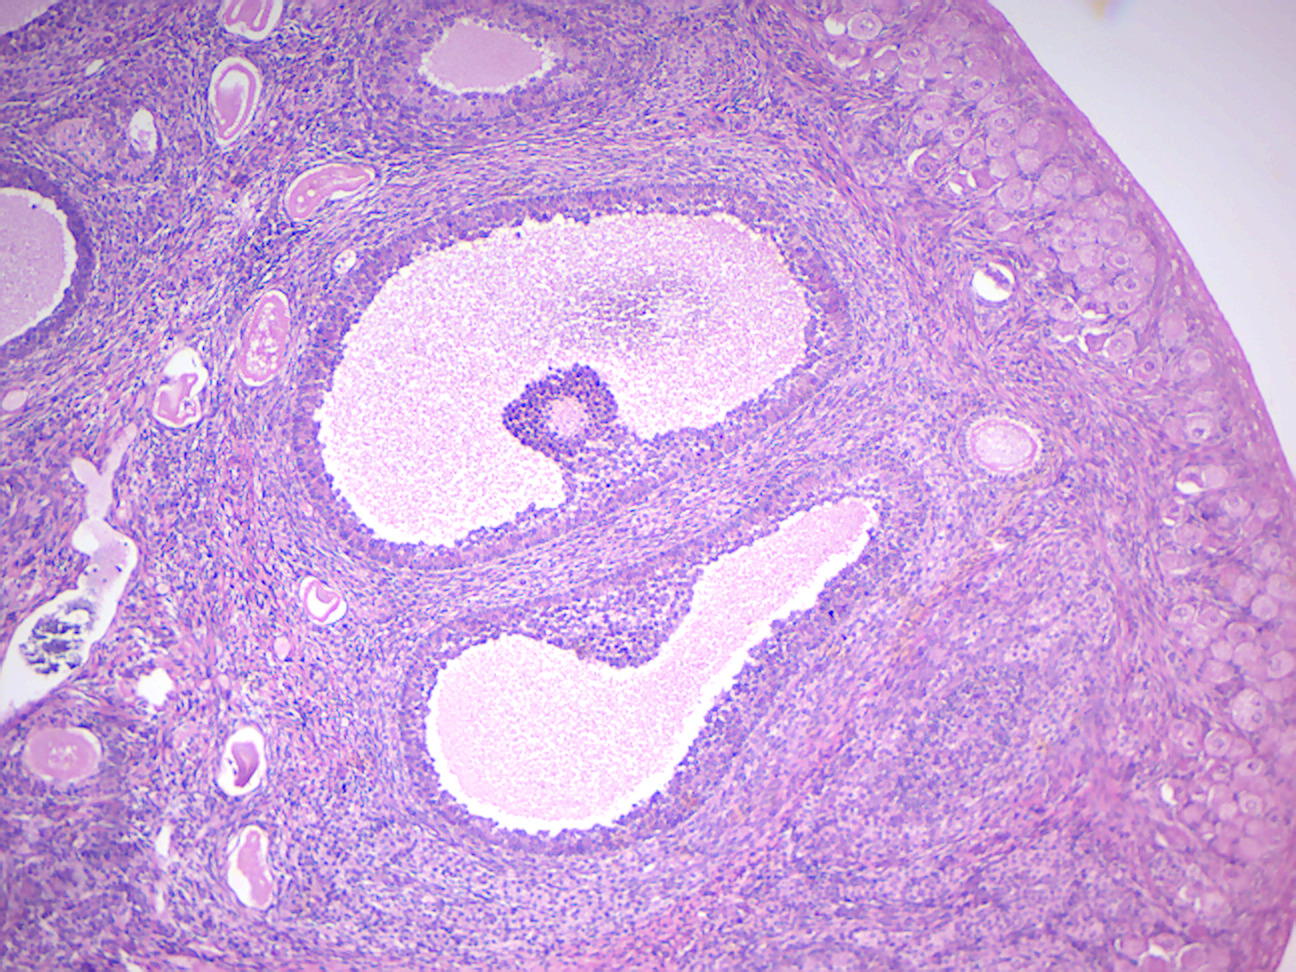
\includegraphics[width=0.7\linewidth]{./figures/development/graafian_follicle}

}

\caption{Graafian follicle in cat ovary.}\label{fig:graafian}
\end{figure}

\begin{figure}

{\centering 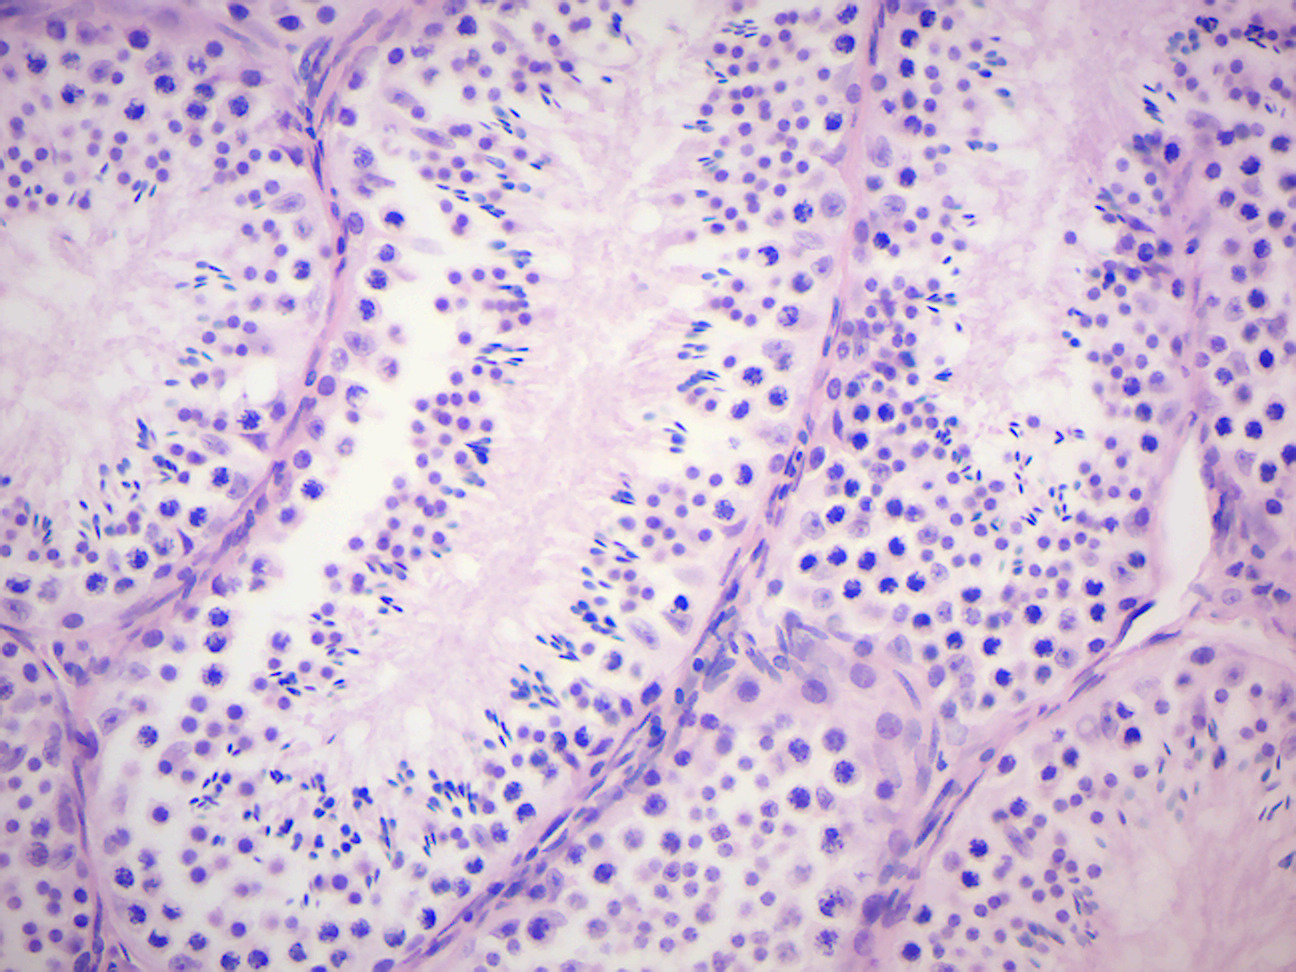
\includegraphics[width=0.7\linewidth]{./figures/development/monkey_testis}

}

\caption{Monkey testis.}\label{fig:monkeytestis}
\end{figure}

\begin{figure}

{\centering 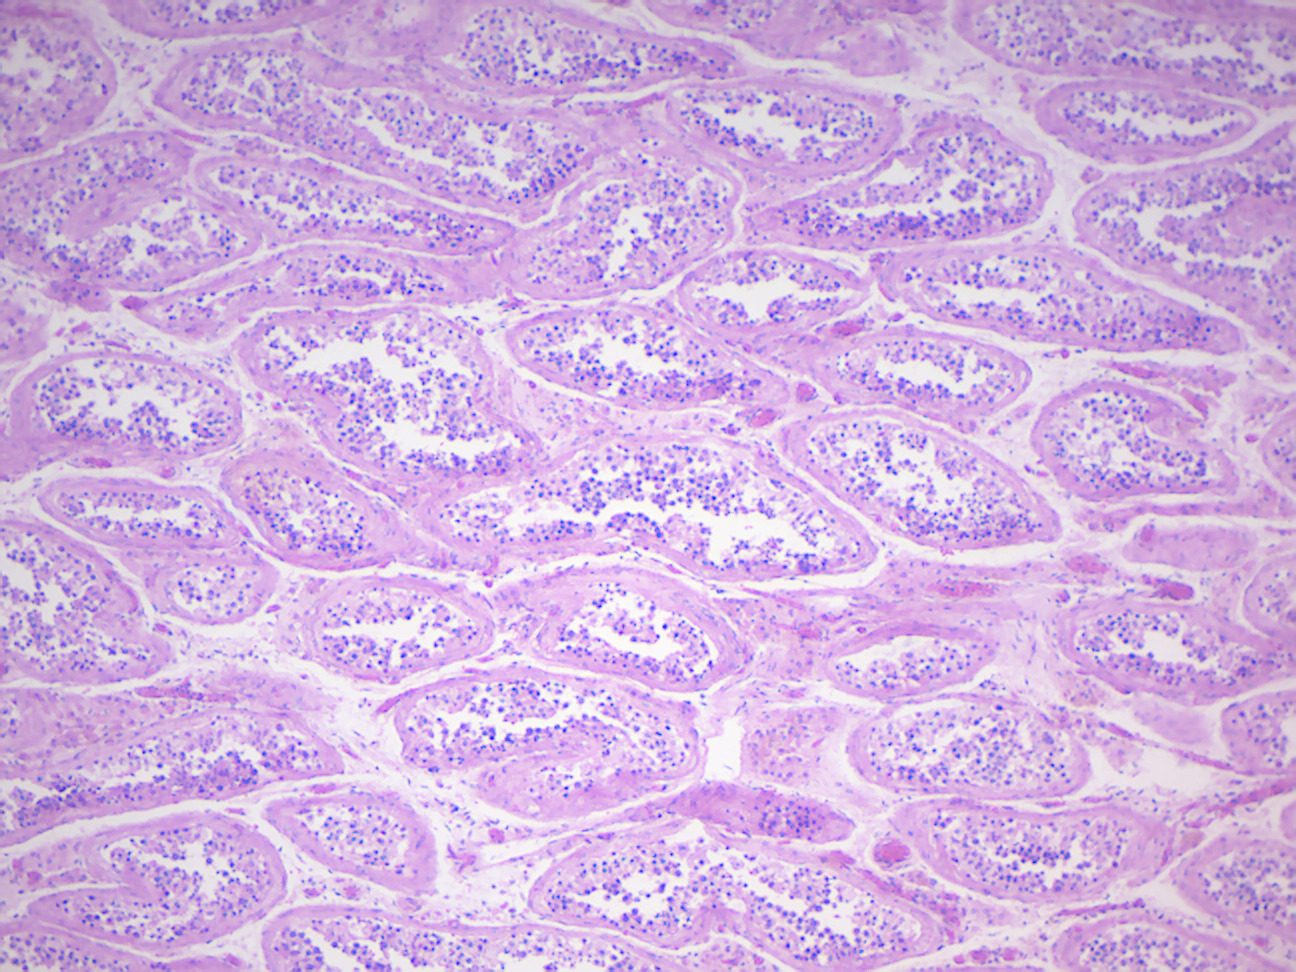
\includegraphics[width=0.7\linewidth]{./figures/development/human_testis}

}

\caption{Human testis.}\label{fig:humantestis}
\end{figure}

\begin{figure}

{\centering 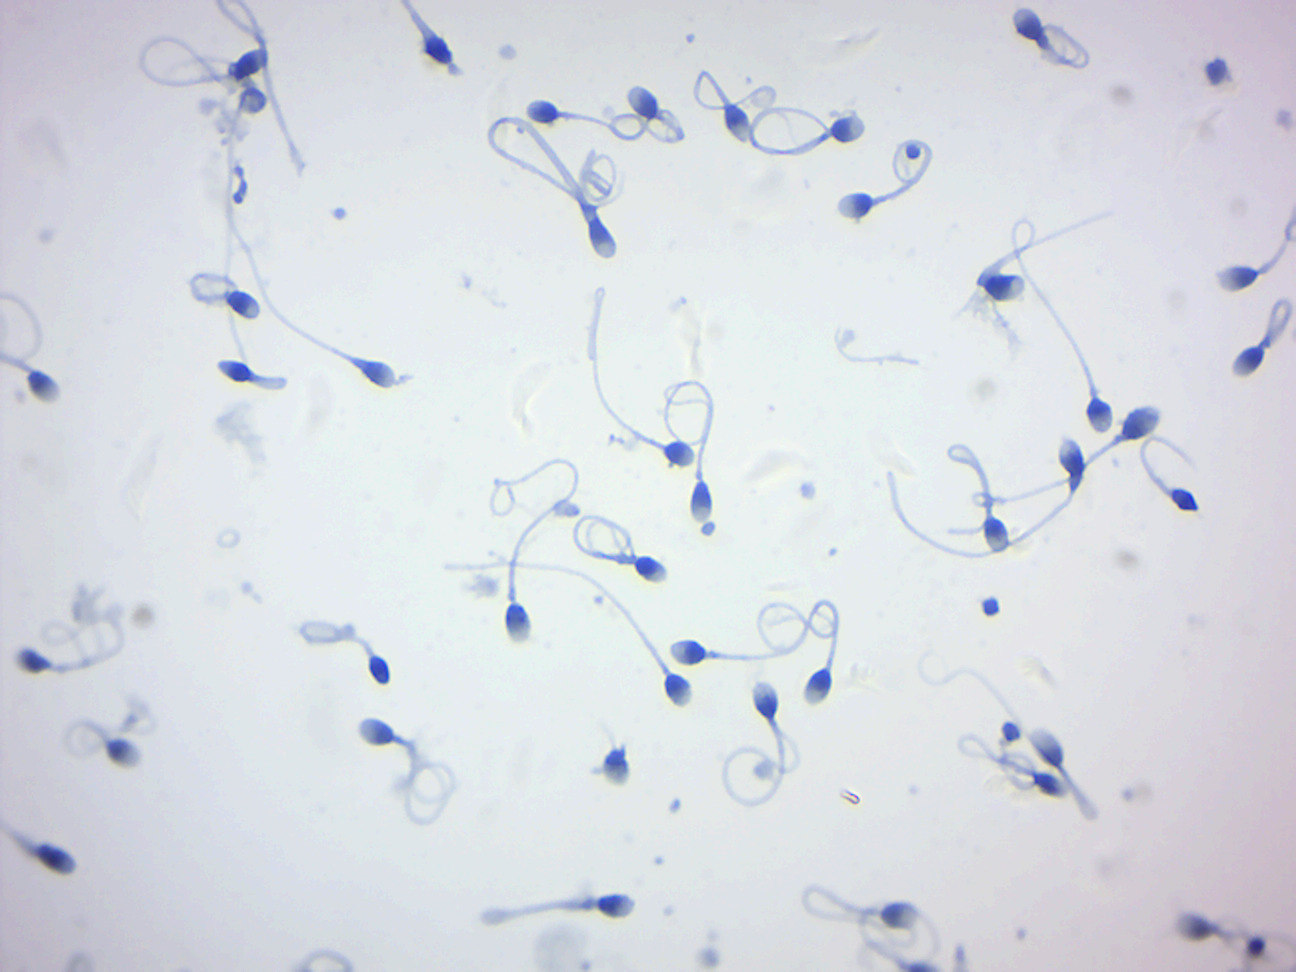
\includegraphics[width=0.7\linewidth]{./figures/development/human_sperm}

}

\caption{Human sperm.}\label{fig:sperm}
\end{figure}

\section{Review Questions}\label{review-questions-10}

\begin{enumerate}
\def\labelenumi{\arabic{enumi}.}
\item
  What are gametes?
\item
  Spermatogenesis is the process in which an animal produces
  \underline{\phantom{answer}}.
\item
  Oogenesis is the process in which an animal produces
  \underline{\phantom{answer}}.
\item
  The gametes fuse to form \underline{\phantom{answer}}, which develop
  via multiple successive mitoses and differentiation into new
  individuals.
\item
  In bilateral animals, the blastula develops in one of two ways that
  divides the whole animal kingdom into two halves.
\item
  If in the blastula the first pore (blastopore) becomes the mouth of
  the animal, it is a \underline{\phantom{answer}}; if the first pore
  becomes the anus then it is a \underline{\phantom{answer}}.
\item
  In triplobastic animals, the three tissue (germ) layers of the
  gastrula are the
\begin{enumerate}
\def\labelenumi{\arabic{enumi}.}
\item
\underline{\phantom{answer}}
\item
\underline{\phantom{answer}}
\item
\underline{\phantom{answer}}
\end{enumerate}
\item
  Somitogenesis is the process by which \underline{\phantom{answer}}
  are produced.
\item
  In frog embryology, what structures are formed during neurulation?
\end{enumerate}
